\documentclass[../main.tex]{subfiles}
\graphicspath{{\subfix{../images/}}}

\usepackage{lipsum}

\begin{document}

\newcommand\getImageWidth{1\linewidth}
\newcommand\getImageHeight{0.3\pdfpageheight}

\section{Demonstracja produktu programowego}
    \subsection{Wstęp}
        W ramach demostracji produktu programowego stworzono przykładowe artykuły, kategorie, magazyny i stany magazynów korzystając z tekstur gry Minecraft. Wszystkie tekstury pochodzą z portalu minecraft.fandom.com \cite{minecraft-images}. Podstawowe widoki zostały przedstawione w dwóch formach: na komputer stacjonarny i na telefon komórkowy. Dla zwięzłości widoki szczegółowe zostały przedstawione tylko w formie na komputer stacjonarny.
    \subsection{Widoki - komputer stacjonarny}
        Podstawowe widoki wyświetlane na komputerze stacjonarnym zostały przedstawione na Rysunkach 
        \ref{fig:app-starting-page-desktop},
        \ref{fig:app-starting-page-after-login-desktop},
        \ref{fig:app-items-desktop}, 
        \ref{fig:app-categories-desktop}, 
        \ref{fig:app-warehouses-desktop}, 
        \ref{fig:app-settings-desktop},
        \ref{fig:app-stock-any-desktop},
        \ref{fig:app-stock-default-desktop}.

    \subsection{Widoki - telefon komórkowy}
    Podstawowe widoki wyświetlane na telefonie komórkowym zostały przedstawione na Rysunkach 
        \ref{fig:app-starting-page-mobile}, 
        \ref{fig:app-starting-page-after-login-mobile}, 
        \ref{fig:app-items-mobile}, 
        \ref{fig:app-categories-mobile}, 
        \ref{fig:app-warehouses-mobile}, 
        \ref{fig:app-settings-mobile},
        \ref{fig:app-stock-any-mobile},
        \ref{fig:app-stock-default-mobile}.

    \subsection{Opis aplikacji}
        \subsubsection{Podstawowe widoki}
            Aplikacja zawiera 7 podstawowych widoków:
            \begin{itemize}
                \item stronę startową (Rysunki \ref{fig:app-starting-page-desktop} i \ref{fig:app-starting-page-mobile}),
                \item artykuły (Rysunki \ref{fig:app-items-desktop} i \ref{fig:app-items-mobile}),
                \item kategorie (Rysunki \ref{fig:app-categories-desktop} i \ref{fig:app-categories-mobile}),
                \item magazyny (Rysunki \ref{fig:app-warehouses-desktop} i \ref{fig:app-warehouses-mobile}),
                \item ustawienia (Rysunki \ref{fig:app-settings-desktop} i \ref{fig:app-settings-mobile})
                \item stany magazynów (Rysunki \ref{fig:app-stock-default-desktop} i \ref{fig:app-stock-default-mobile}),
                \item skaner kodów kreskowych i kodów QR. 
            \end{itemize}
        
        \subsubsection{Strona startowa}
            Strona startowa może przyjąć 2 stany: użytkownik niezalogowany (Rysunek \ref{fig:app-starting-page-desktop}) i użytkownik zalogowany (Rysunek \ref{fig:app-starting-page-after-login-desktop}).
            W przypadku użytkownika niezalogowanego jedyną funkcjonalnością jest przekierowanie do logowania.
            W przypadku użytkownika zalogowanego istnieją dwie funkcjonalności: wylogowanie lub przejście do aplikacji.

            Po poprawnej próbie zalogowania użytkownik zostaje automatycznie przekierowany do aplikacji. Jeśli kiedykolwiek ponownie znajdzie się na stronie startowej to dostanie możliwość przejścia do aplikacji ręcznie lub możliwość wylogowania się. Po wylogowaniu użytkownik zostaje przekierowany z powrotem na stronę startową.

            \begin{figure}[H]
                \centering
                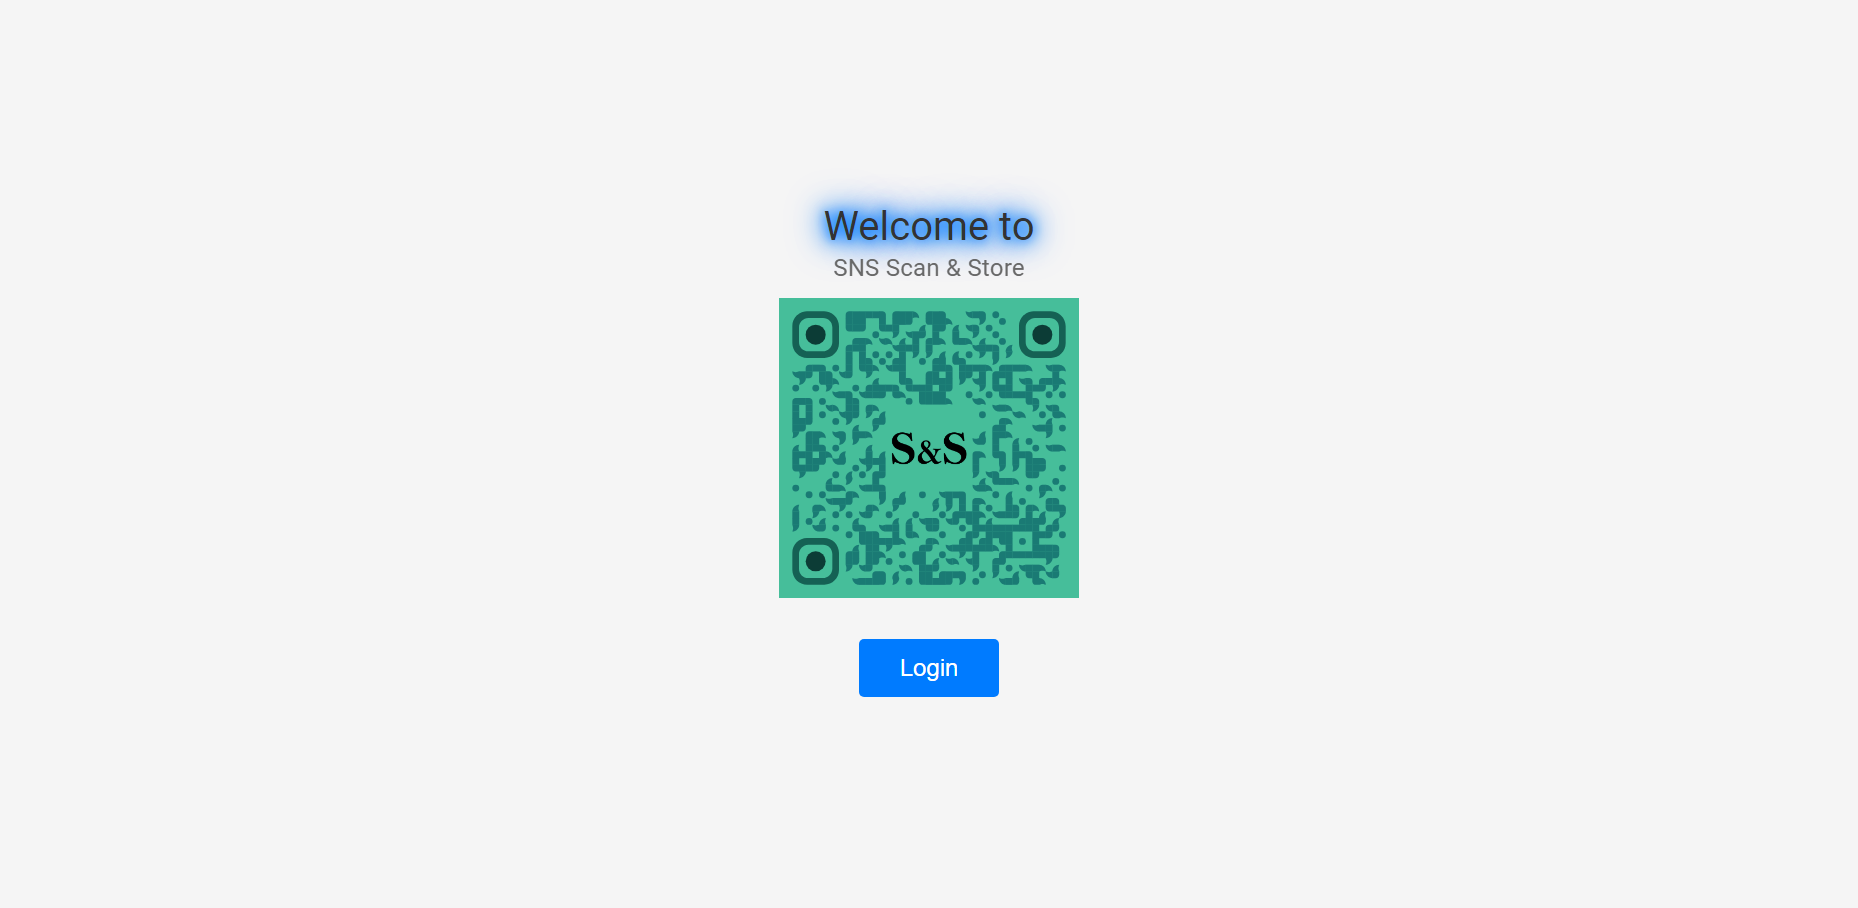
\includegraphics[width=\getImageWidth]{images/app-desktop/app-starting-page-desktop.png}
                \caption{Strona startowa na komputerze stacjonarnym}
                \label{fig:app-starting-page-desktop}
            \end{figure}
            \begin{figure}[H]
                \centering
                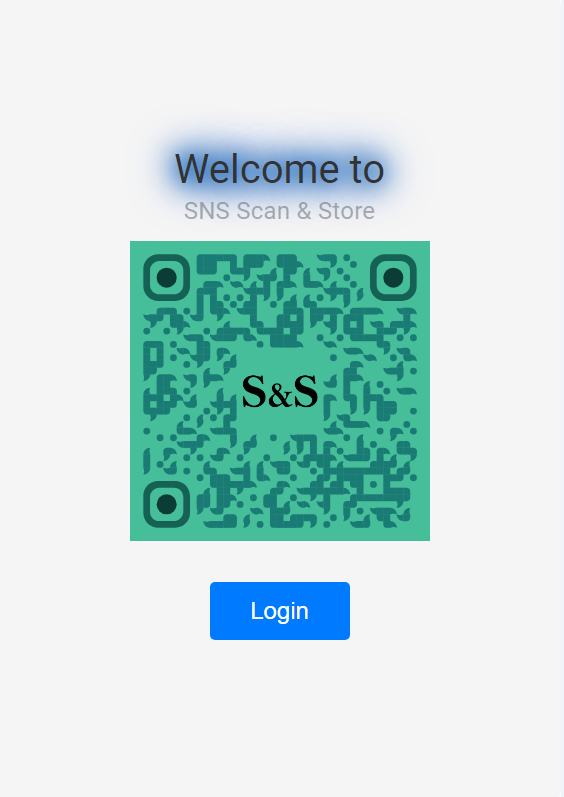
\includegraphics[height=\getImageHeight]{images/app-mobile/app-starting-page-mobile.png}
                \caption{Strona startowa na telefonie komórkowym}
                \label{fig:app-starting-page-mobile}
            \end{figure}

            \begin{figure}[H]
                \centering
                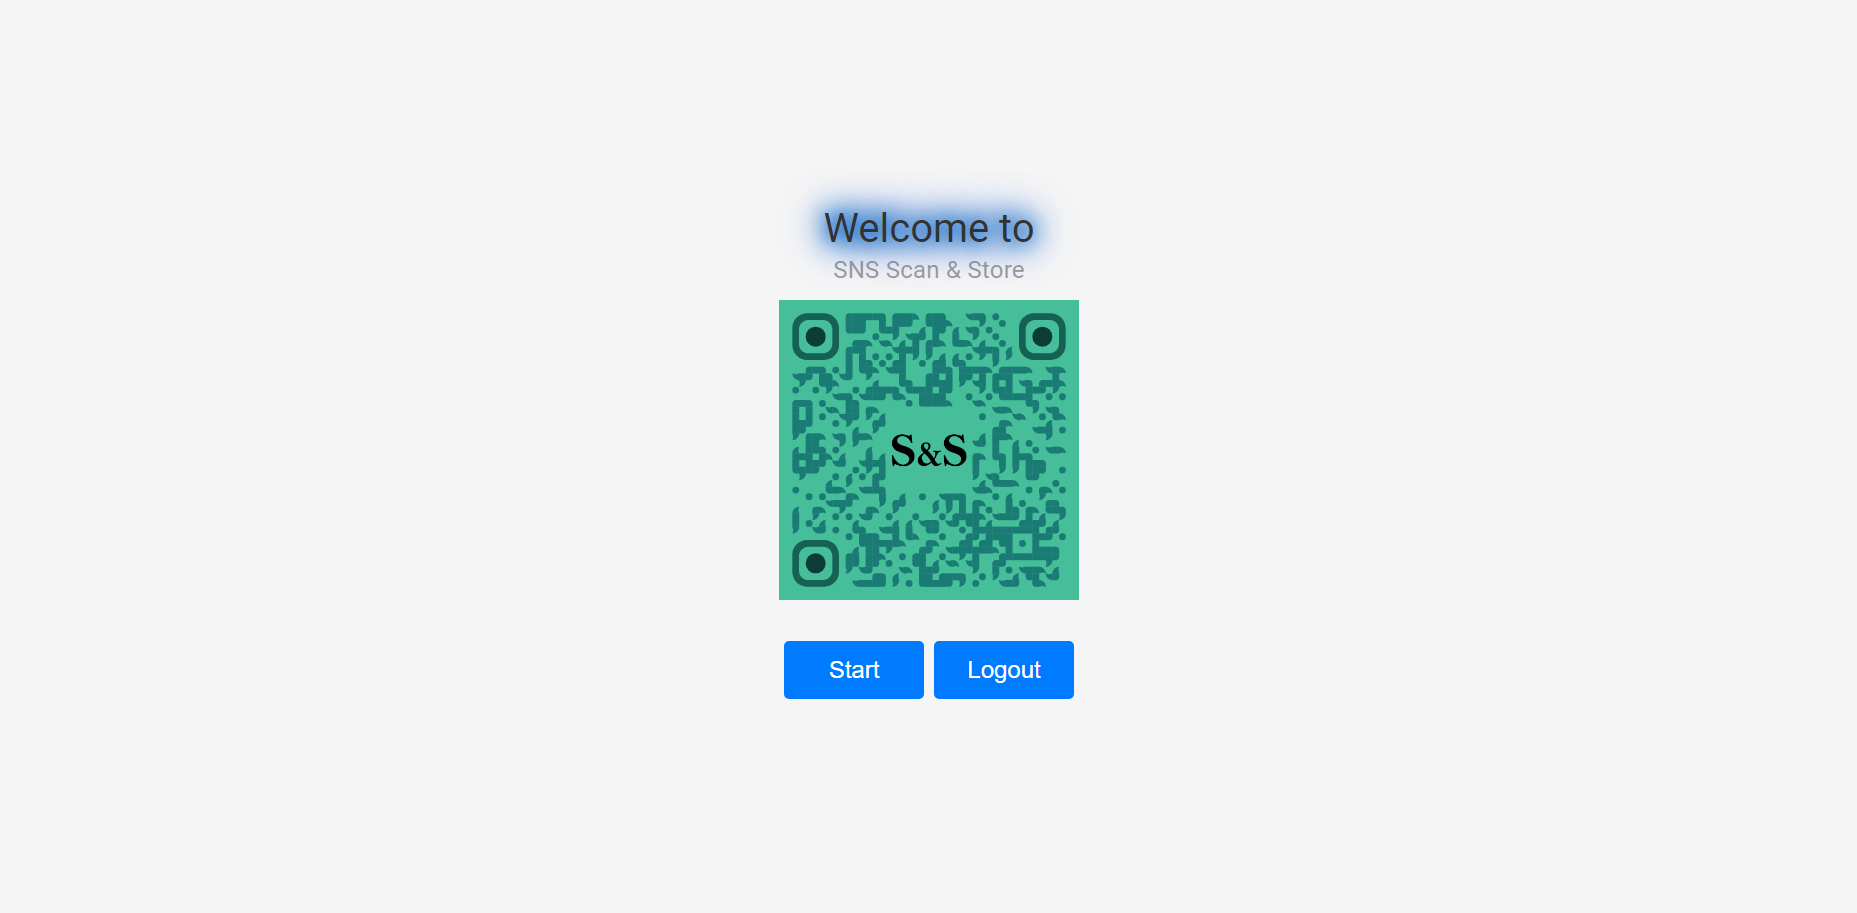
\includegraphics[width=\getImageWidth]{images/app-desktop/app-starting-page-after-login-desktop.png}
                \caption{Strona startowa po zalogowaniu na komputerze stacjonarnym}
                \label{fig:app-starting-page-after-login-desktop}
            \end{figure}
            \begin{figure}[H]
                \centering
                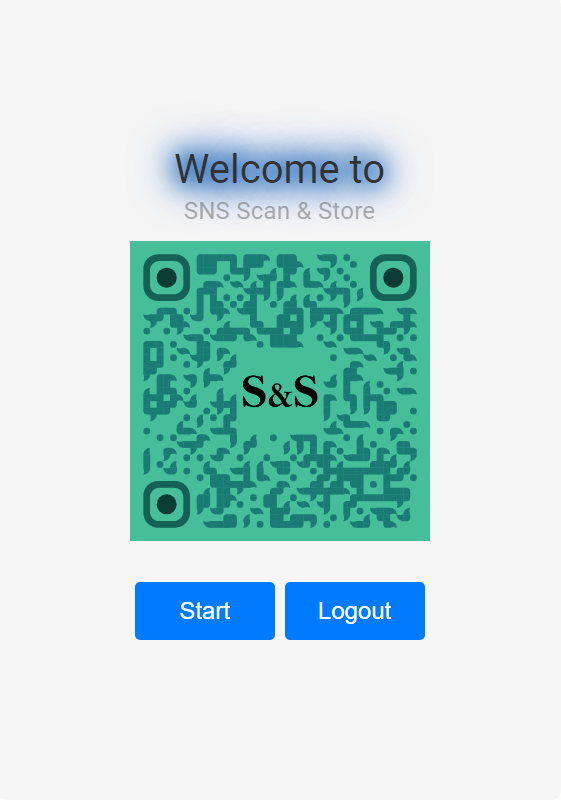
\includegraphics[height=\getImageHeight]{images/app-mobile/app-starting-page-after-login-mobile.png}
                \caption{Strona startowa po zalogowaniu na telefonie komórkowym}
                \label{fig:app-starting-page-after-login-mobile}
            \end{figure}

        \FloatBarrier 
        \subsubsection{Artykuły}
            Strona artykułów przedstawiona na rysunku \ref{fig:app-items-desktop} służy do pełnej obsługi wszystkich dostępnych artykułów, które mogą znaleźć się w dowolonym magazynie. W górnym pasku znajdują się opcje pozwalające na kolejno od lewej:
            \begin{itemize}
                \item przejście z powrotem do strony startowej (element wspólny dla wszystkich widoków)
                \item wyszukanie konkretnego artykułu z uwzględnieniem nazwy i nazwy kategorii
                \item posortowanie artykułów względem nazwy
                \item dodanie nowego artykułu
                \item przejście do widoku ustawień (element wspólny dla wszystkich widoków)
            \end{itemize}
            Wybór konkretnego artykułu następuje poprzez naciśnięcie na konkretny wpis. Po wyborze użytkownik jest przeniesiony do strony ze szczegółami artykułu (Rysunek \ref{fig:app-items-details-desktop}), a w górnym pasku otrzymuje możliwość edycji i usunięcia danego artykułu. 
            
            \begin{figure}[H]
                \centering
                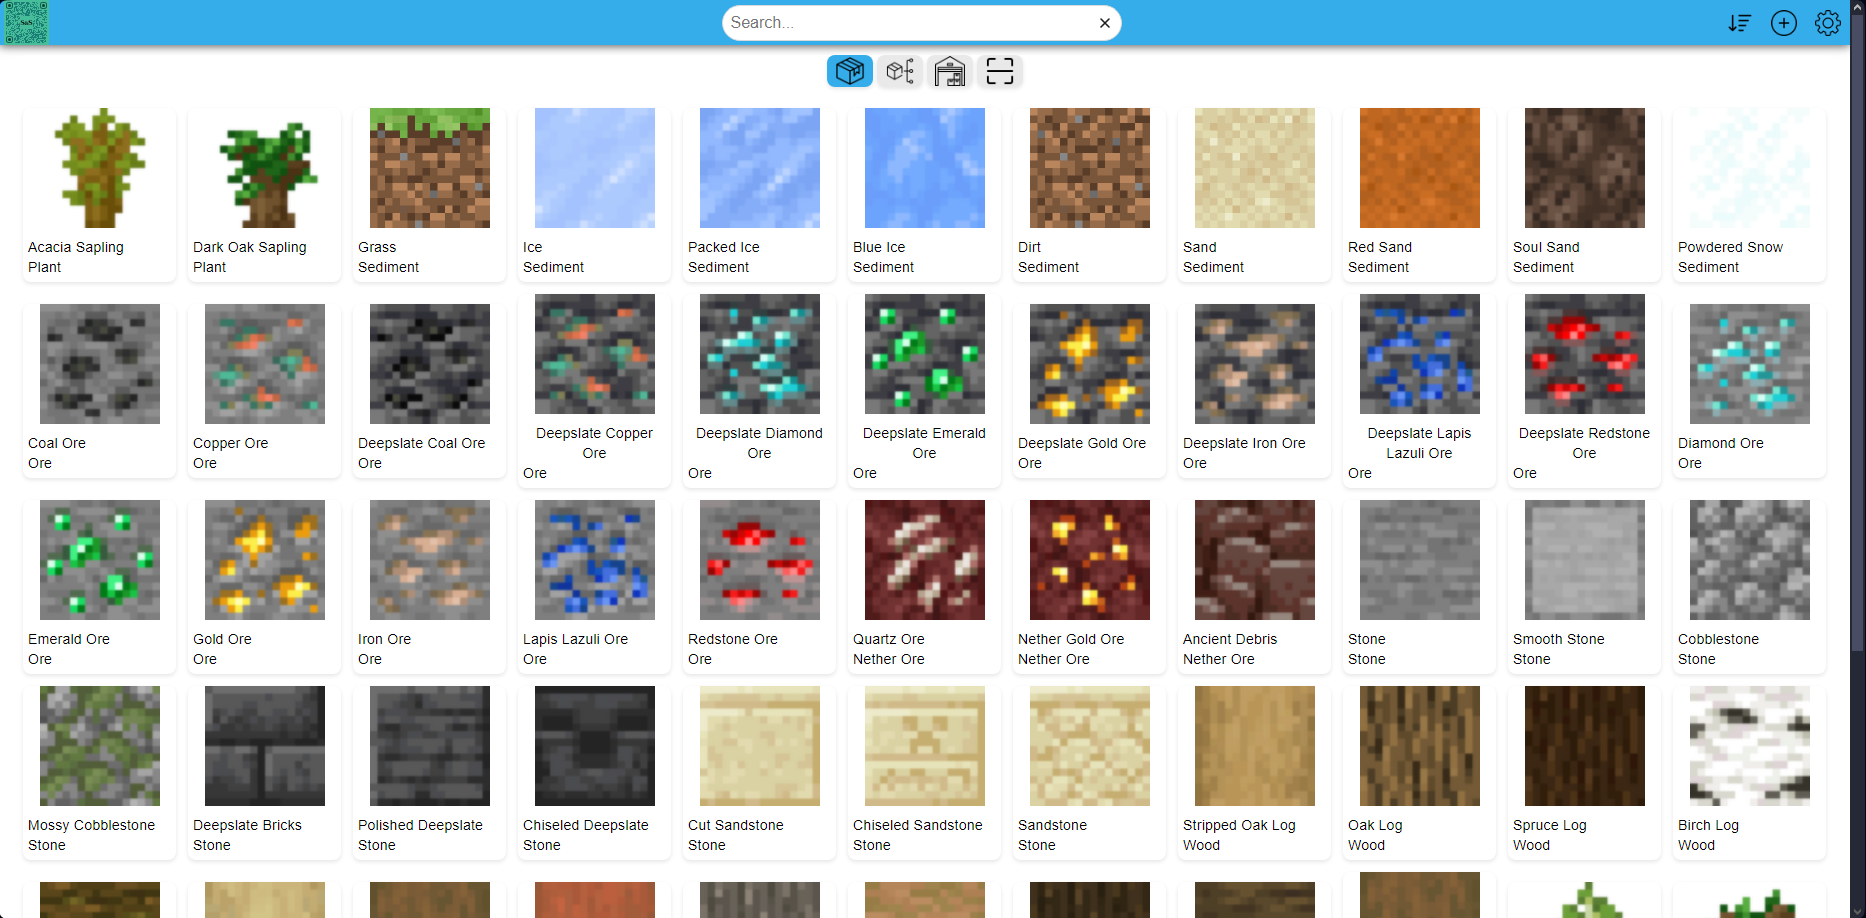
\includegraphics[width=\getImageWidth]{images/app-desktop/app-items-desktop.png}
                \caption{Widok przedmiotów na komputerze stacjonarnym}
                \label{fig:app-items-desktop}
            \end{figure}
            
            \begin{figure}[H]
                \centering
                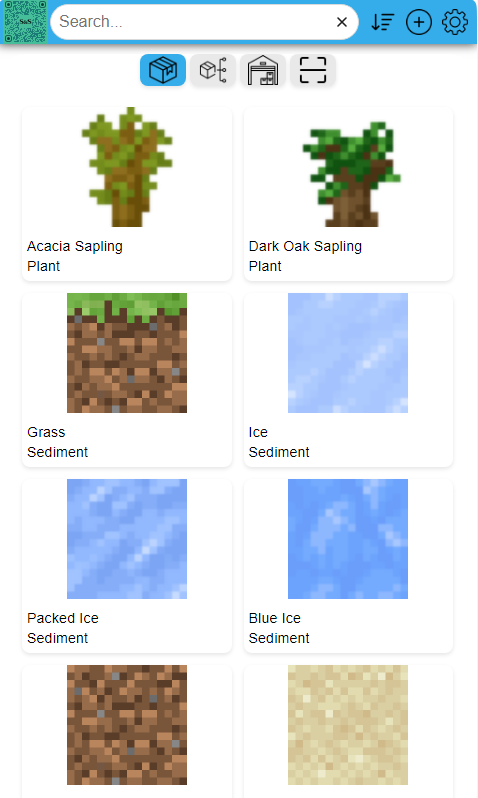
\includegraphics[height=\getImageHeight]{images/app-mobile/app-items-mobile.png}
                \caption{Widok przedmiotów na telefonie komórkowym}
                \label{fig:app-items-mobile}
            \end{figure}

            \begin{figure}[H]
                \begin{subfigure}{.49\textwidth}
                    \centering
                    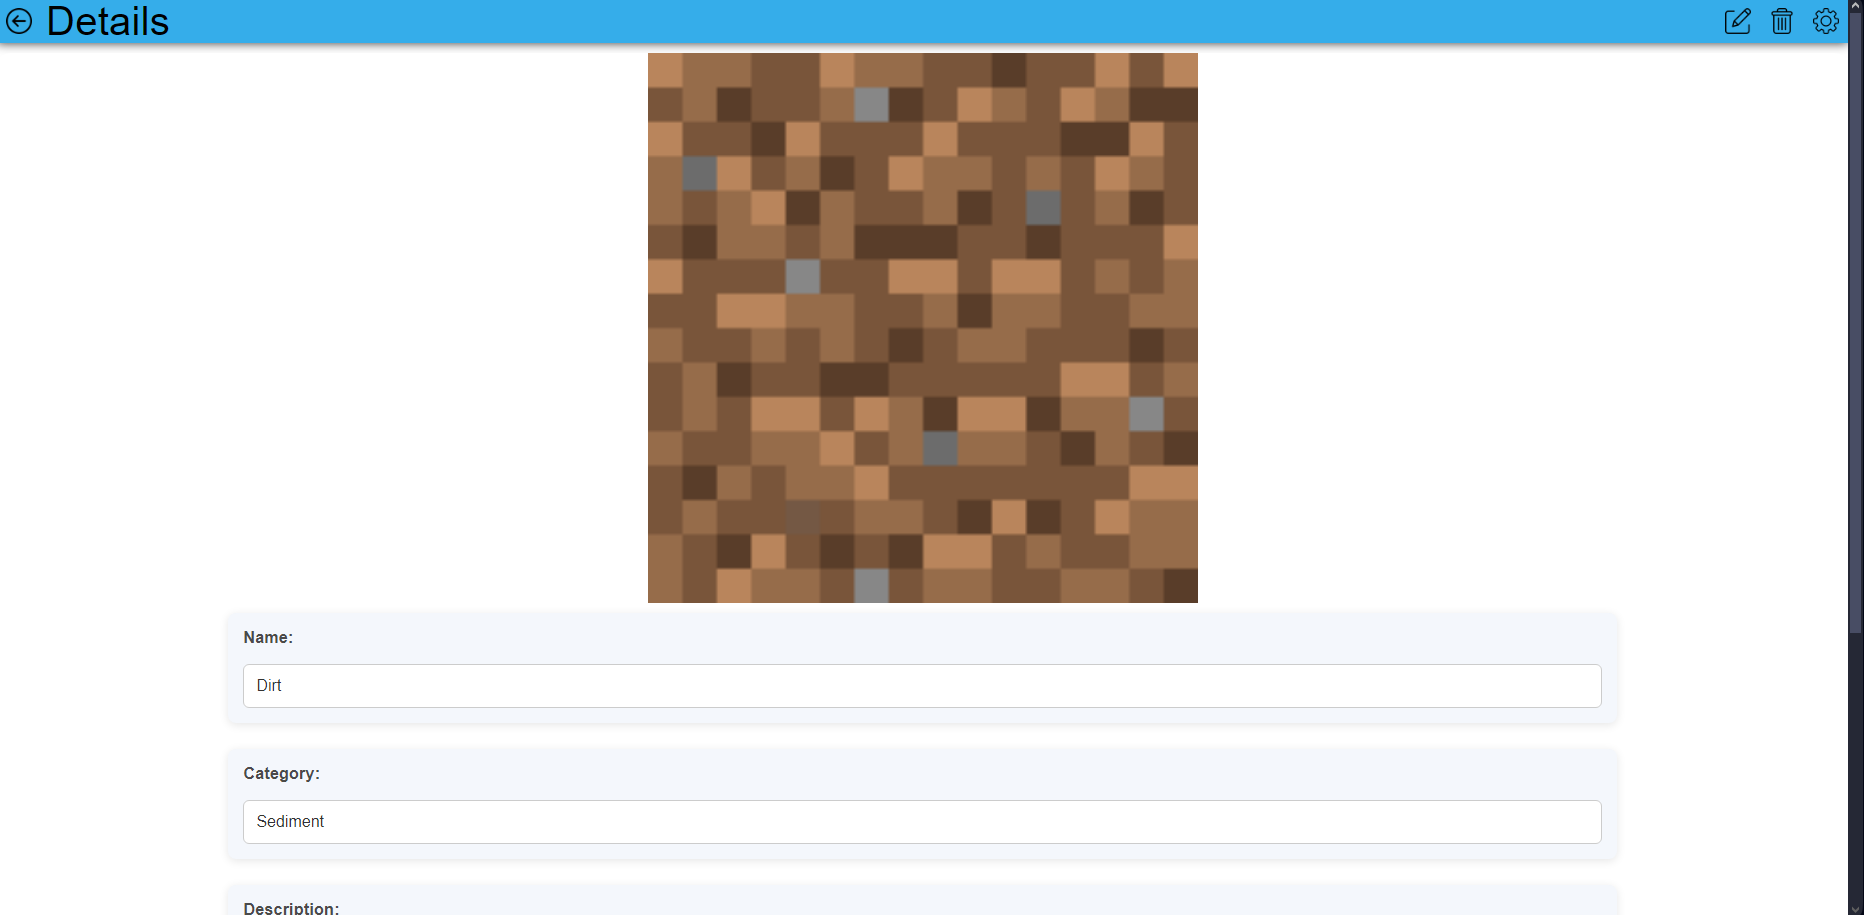
\includegraphics[width=\getImageWidth]{images/app-desktop/app-items-details1-desktop.png}
                    \label{fig:app-items-details1-desktop}
                \end{subfigure}
                \begin{subfigure}{.49\textwidth}
                    \centering
                    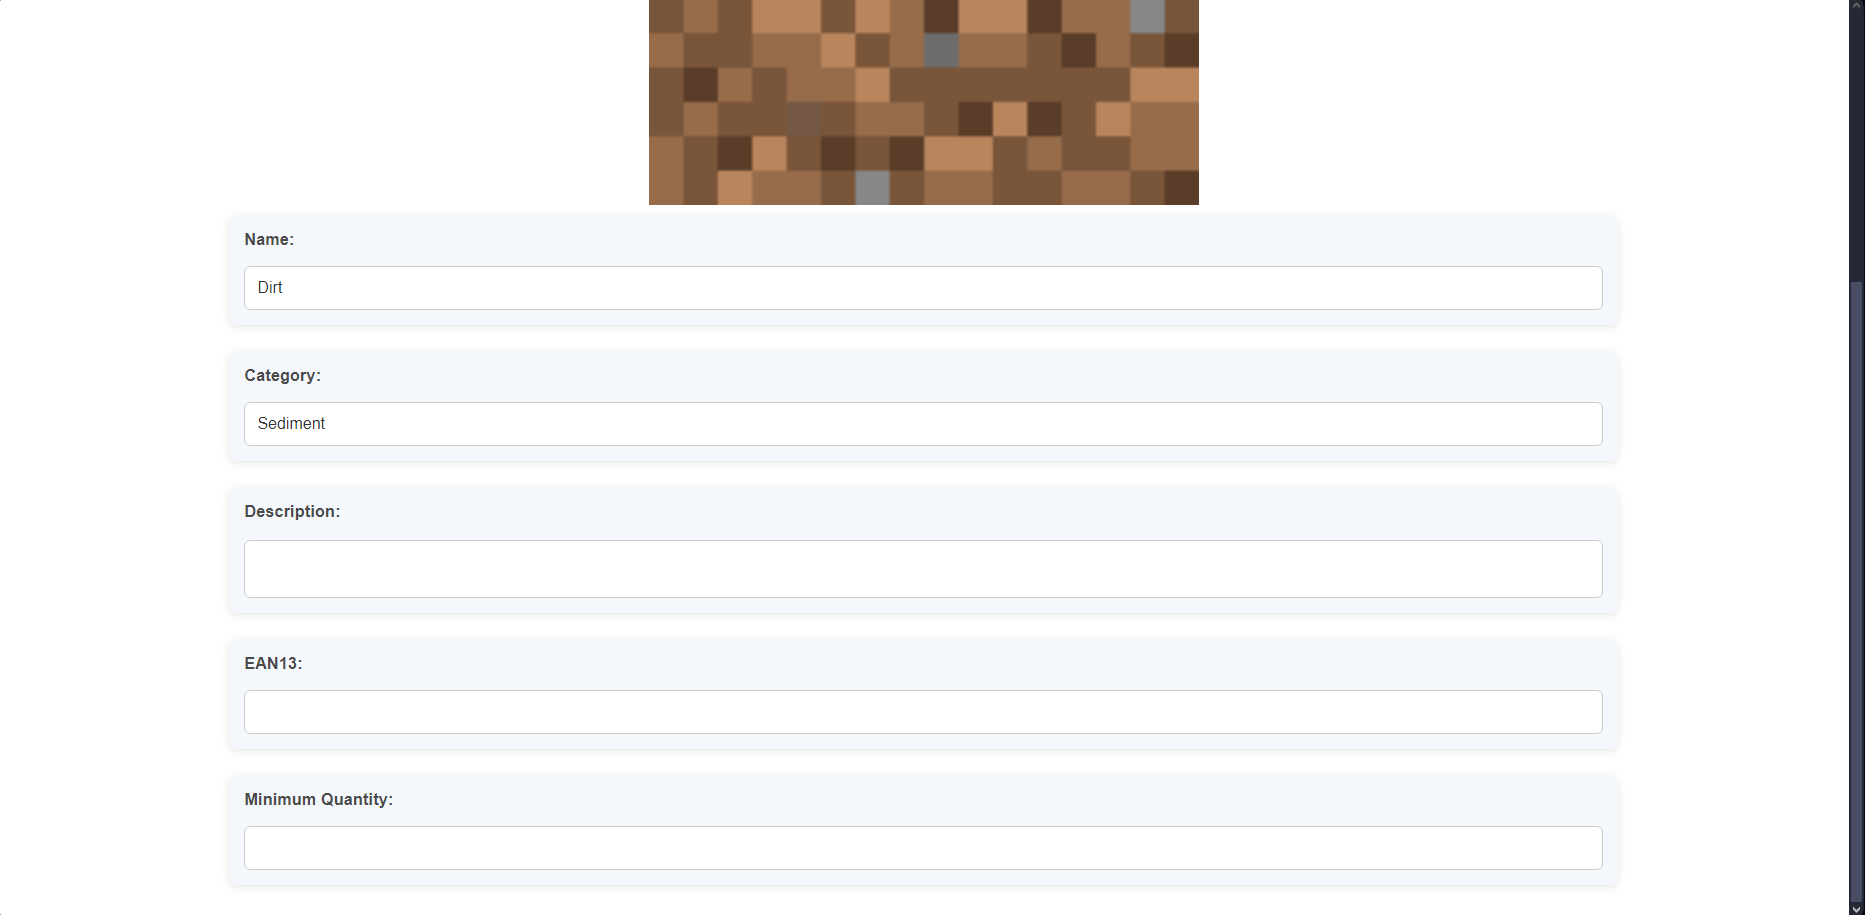
\includegraphics[width=\getImageWidth]{images/app-desktop/app-items-details2-desktop.png}
                    \label{fig:app-items-details2-desktop}
                \end{subfigure}
                \caption{Widok szczegółów przedmiotu}
                \label{fig:app-items-details-desktop}
            \end{figure}
            
            W widoku edycji (Rysunek \ref{fig:app-items-edit-desktop}) użytkownik może zmienić dowolny element dotyczący artykułu, włącznie z dodaniem lub usunięciem zdjęcia.
            \begin{figure}[H]
                \begin{subfigure}{.49\textwidth}
                    \centering
                    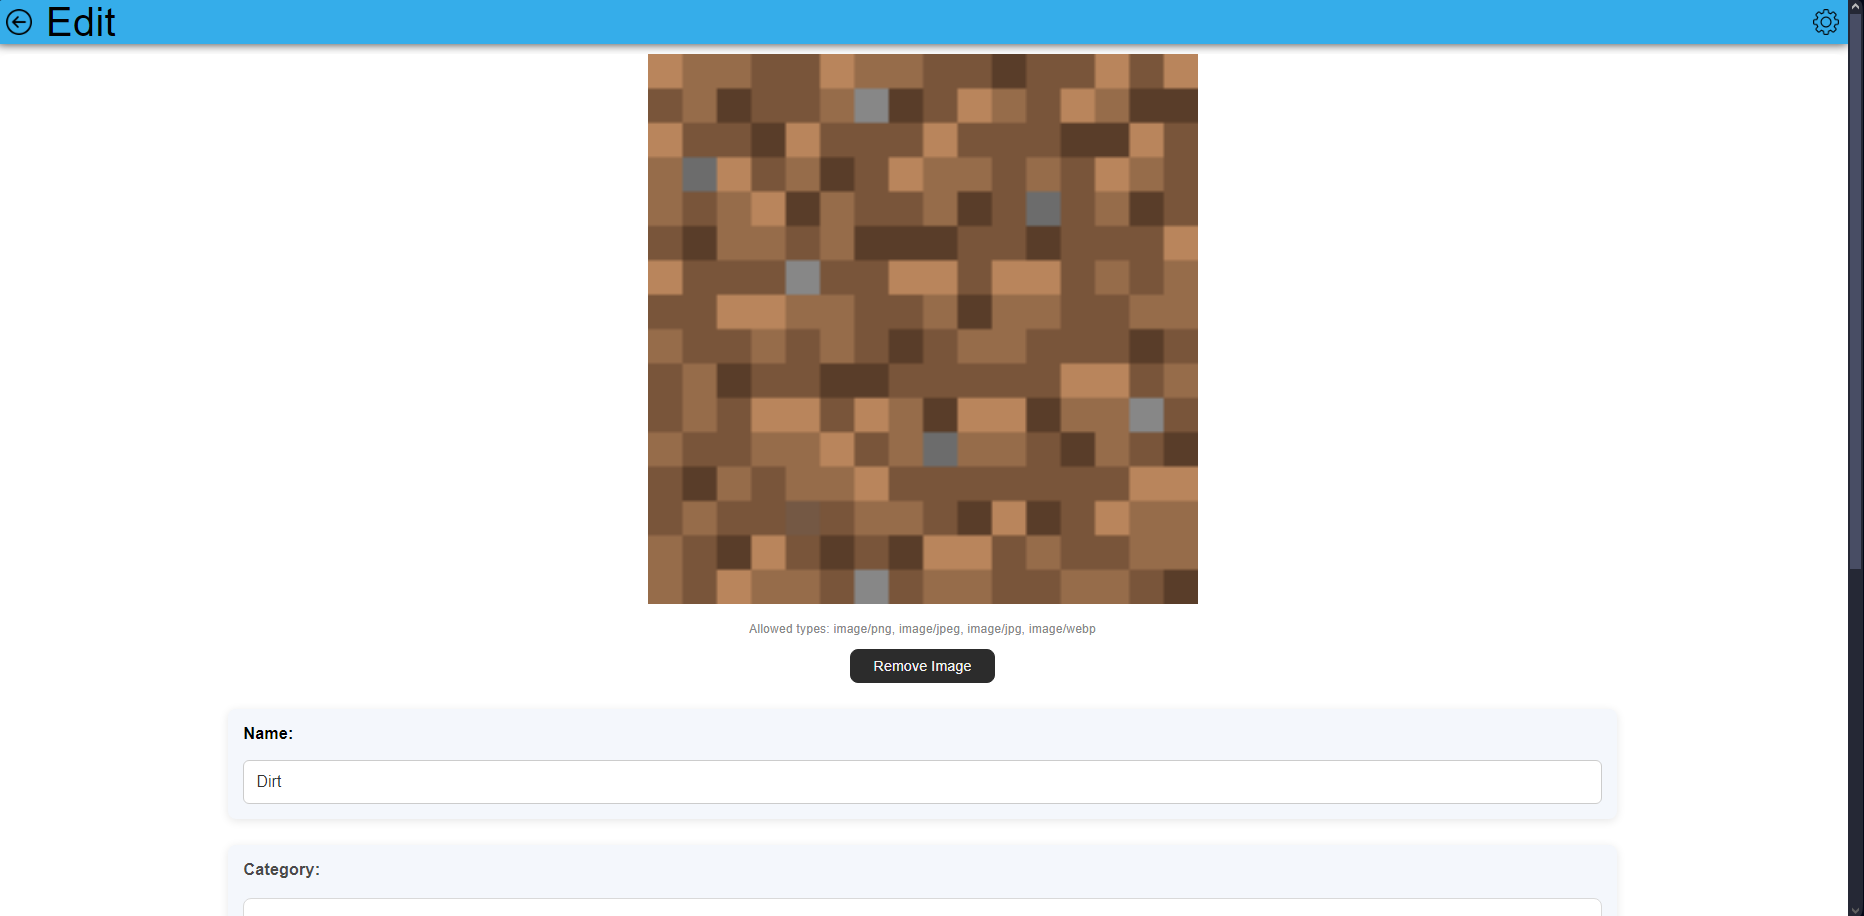
\includegraphics[width=\getImageWidth]{images/app-desktop/app-items-edit1-desktop.png}
                    \label{fig:app-items-edit1-desktop}
                \end{subfigure}
                \begin{subfigure}{.49\textwidth}
                    \centering
                    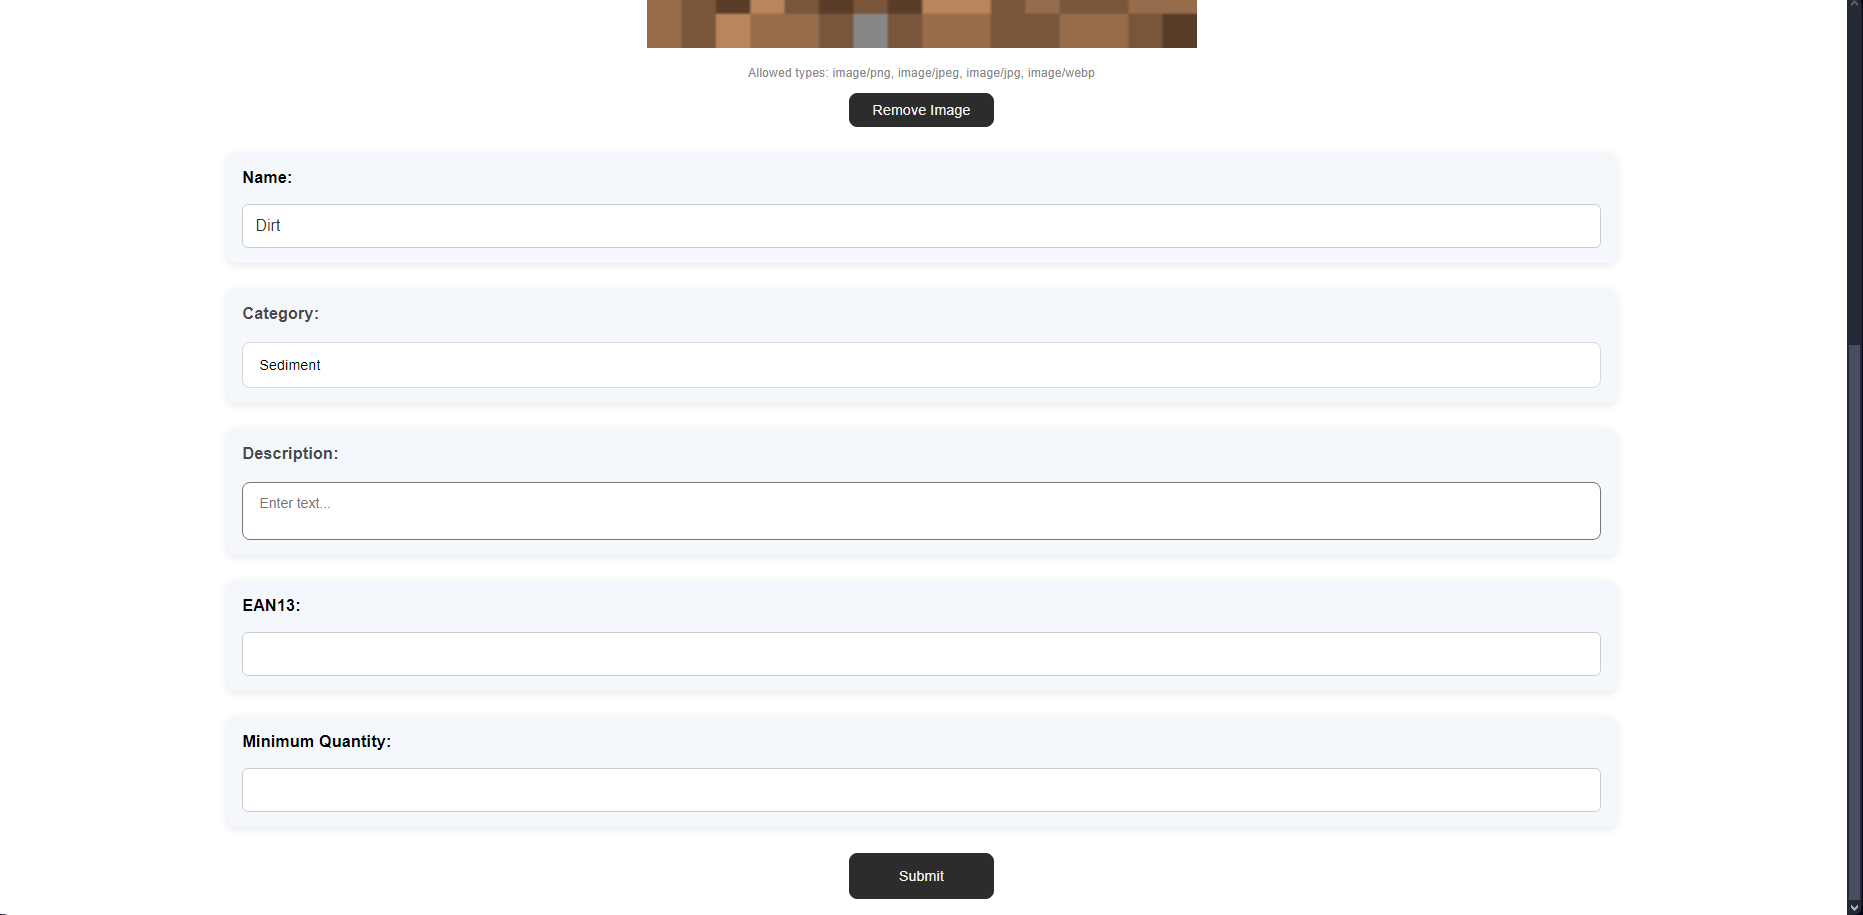
\includegraphics[width=\getImageWidth]{images/app-desktop/app-items-edit2-desktop.png}
                    \label{fig:app-items-edit2-desktop}
                \end{subfigure}
                \caption{Widok edycji przedmiotu}
                \label{fig:app-items-edit-desktop}
            \end{figure}
            
            Po przejściu do widoku dodawania nowego przedmiotu otrzymamy widok, przedstawiony na Rysunku \ref{fig:app-items-add-desktop}, który pozwala na dokładnie te same funkcjonalności co edycja, lecz na początku nie posiada żadnych wypełnionych pól.
            \begin{figure}[H]
                \begin{subfigure}{.49\textwidth}
                    \centering
                    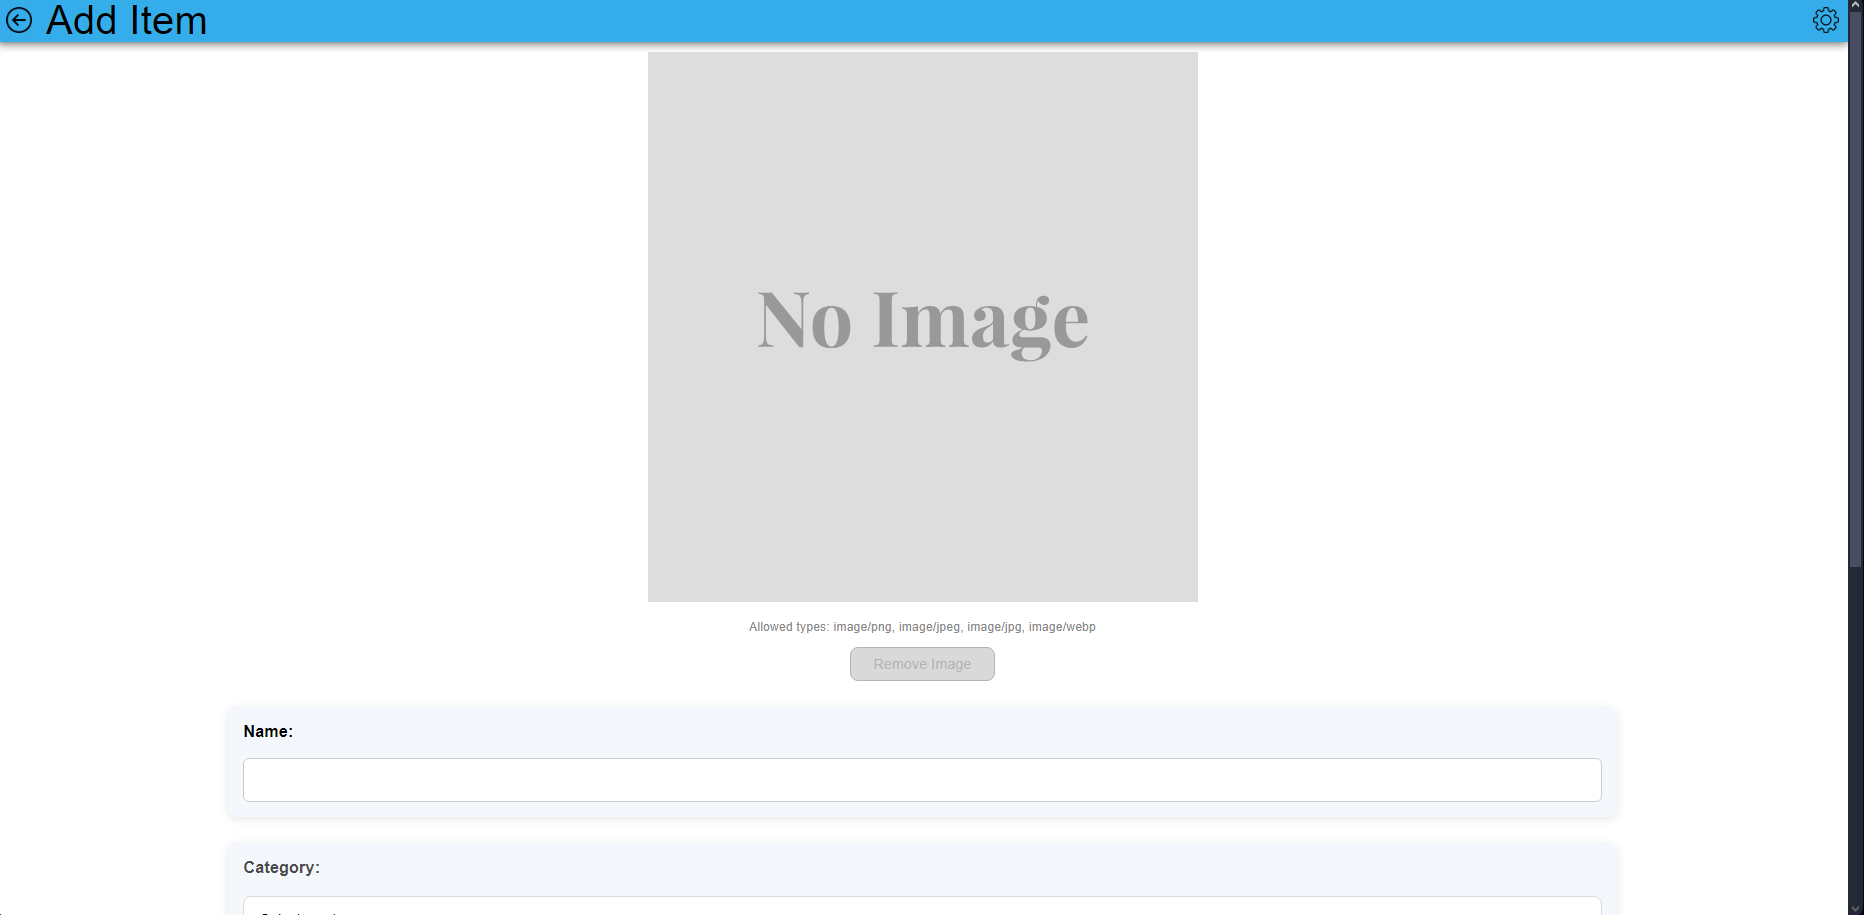
\includegraphics[width=\getImageWidth]{images/app-desktop/app-items-add1-desktop.png}
                    \label{fig:app-items-add1-desktop}
                \end{subfigure}
                \begin{subfigure}{.49\textwidth}
                    \centering
                    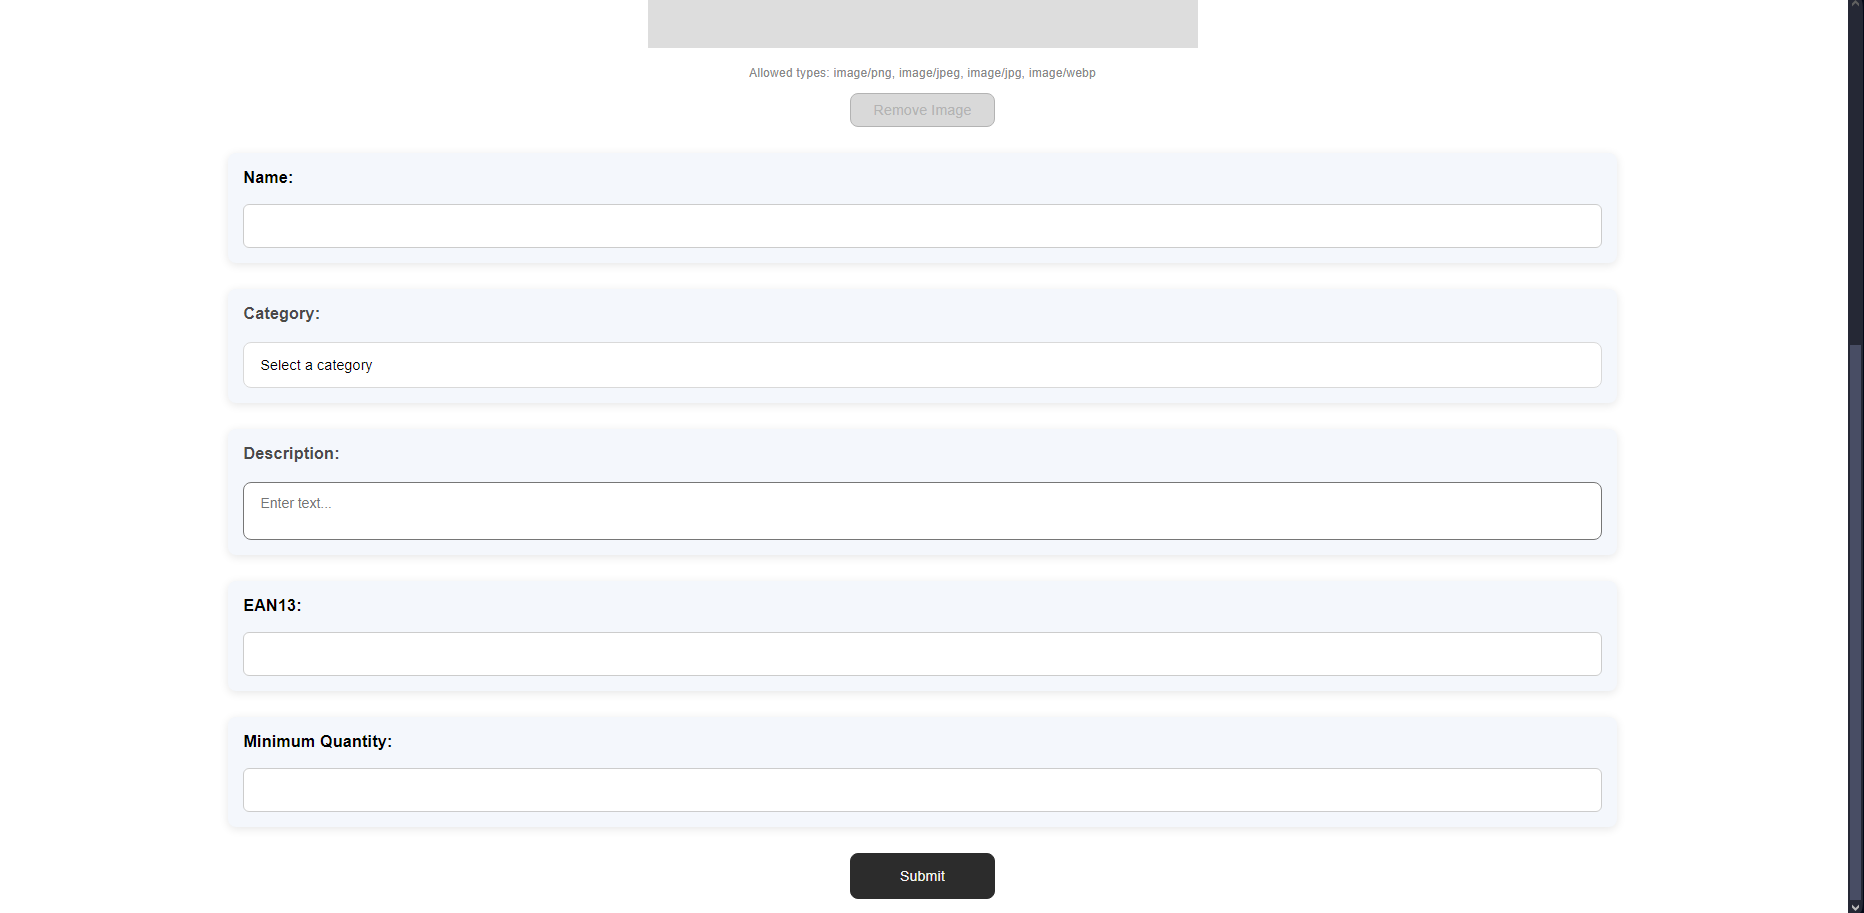
\includegraphics[width=\getImageWidth]{images/app-desktop/app-items-add2-desktop.png}
                    \label{fig:app-items-add2-desktop}
                \end{subfigure}
                \caption{Widok dodawania przedmiotu}
                \label{fig:app-items-add-desktop}
            \end{figure}

        \FloatBarrier 
        \subsubsection{Kategorie}
            Strona kategorii przedstawiona na rysunku \ref{fig:app-categories-desktop} pozwala na przegląd i dodawanie kategorii dla przedmiotów. Podobnie jak w przypadku artykułów w pasku górnym znajdują się te same opcje. Także analogicznie do artykułów wybór kategorii następuje poprzez nacisnięcie odpowiedniego elementu.

            Widok szczegółow (Rysunek \ref{fig:app-categories-details-desktop}), edycji (Rysunek \ref{fig:app-categories-edit-desktop}) i dodawania (Rysunek \ref{fig:app-categories-add-desktop}) nowej kategorii działa tak samo jak w przypadku artykułów.

            \begin{figure}[H]
                \centering
                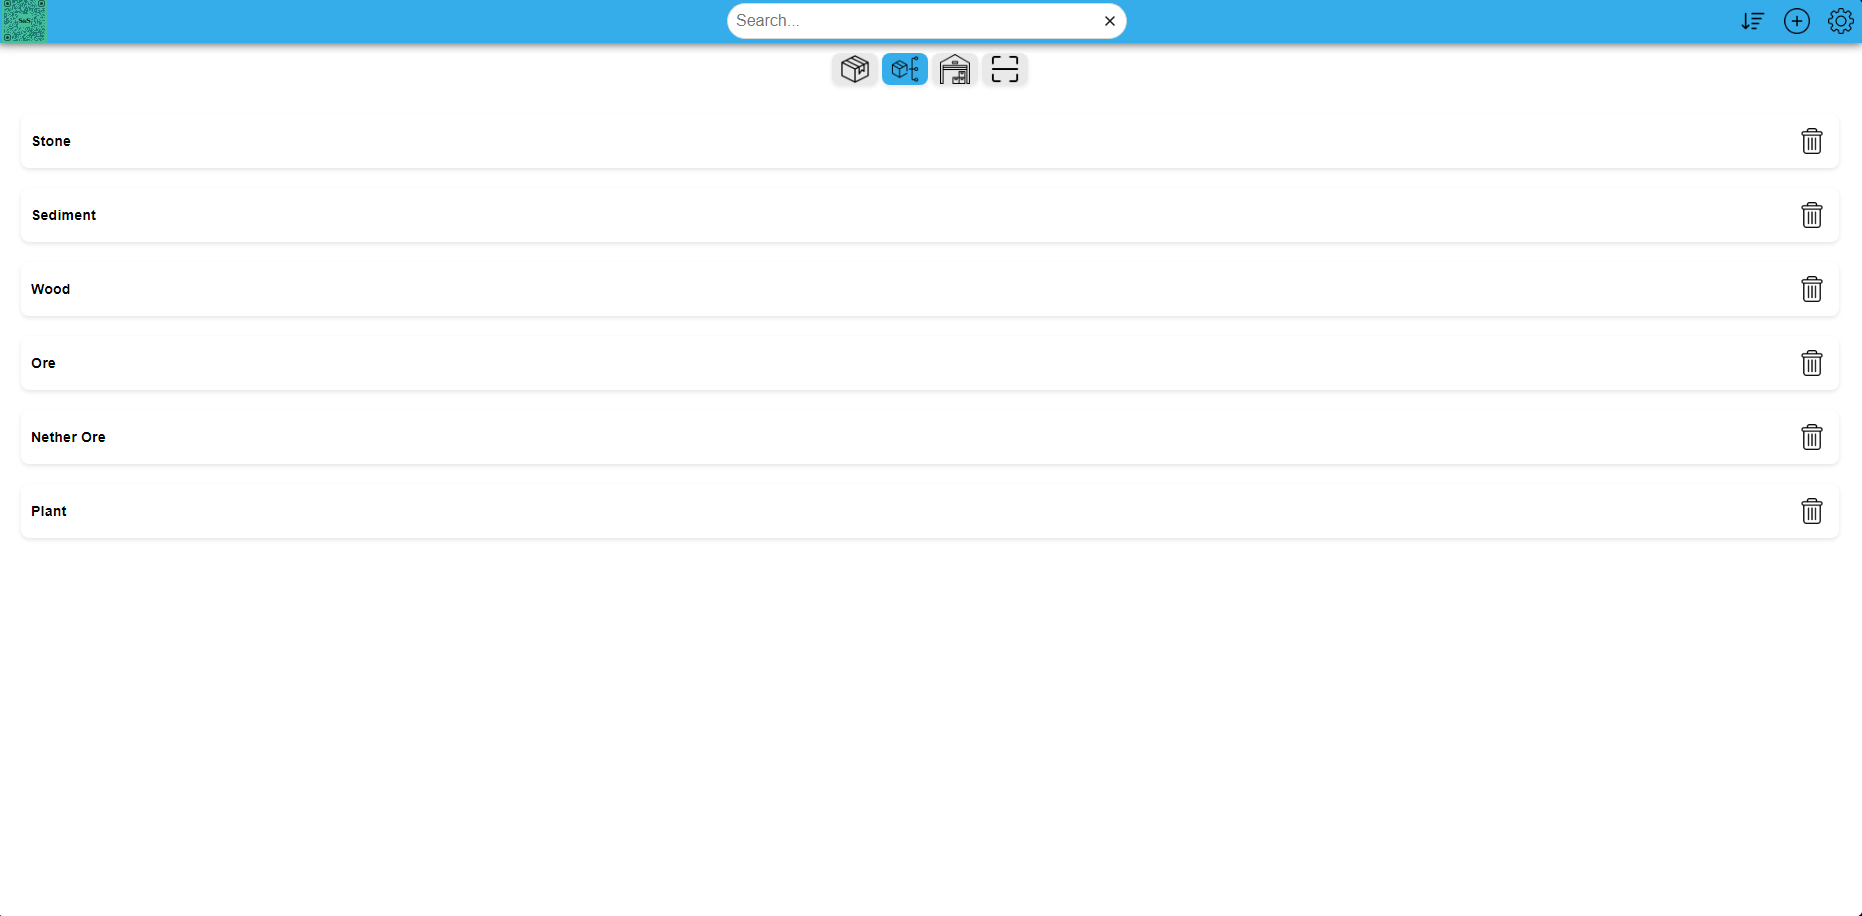
\includegraphics[width=\getImageWidth]{images/app-desktop/app-categories-desktop.png}
                \caption{Widok kategorii na komputerze stacjonarnym}
                \label{fig:app-categories-desktop}
            \end{figure}

            \begin{figure}[H]
                \centering
                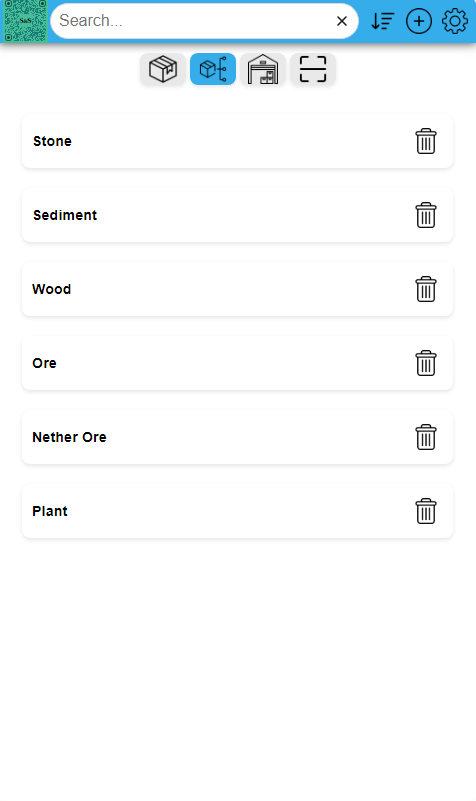
\includegraphics[height=\getImageHeight]{images/app-mobile/app-categories-mobile.png}
                \caption{Widok kategorii na telefonie komórkowym}
                \label{fig:app-categories-mobile}
            \end{figure}

            \begin{figure}[H]
                \centering
                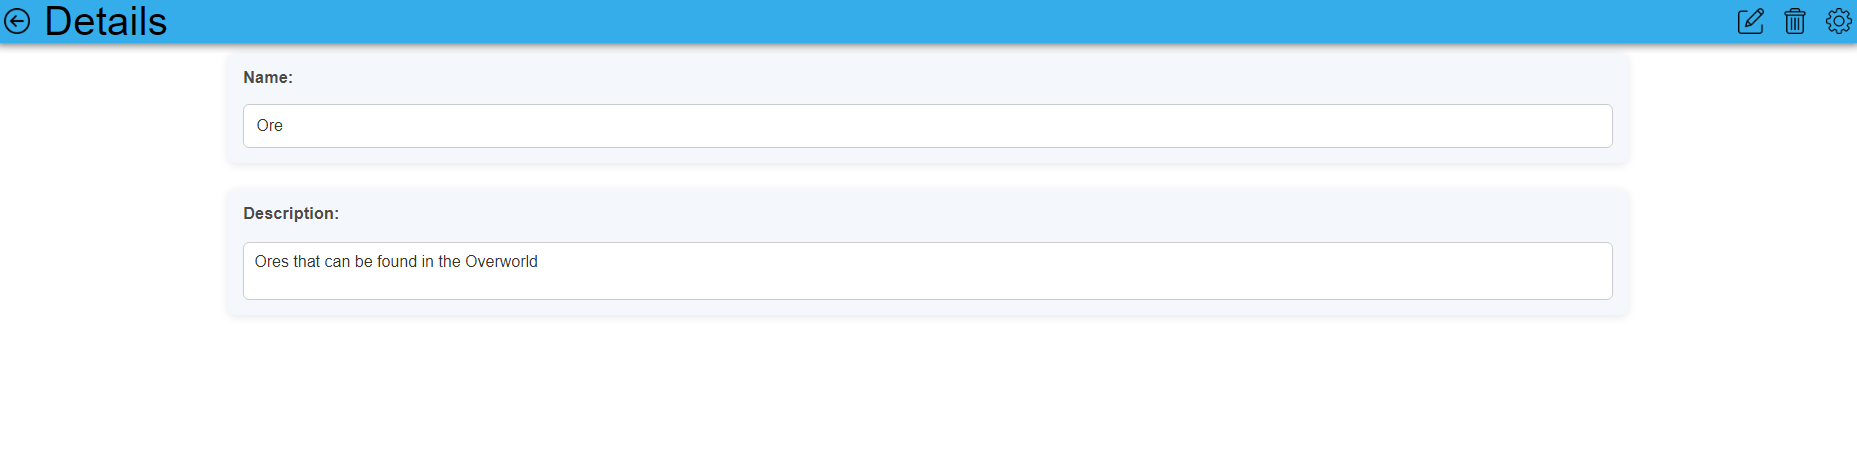
\includegraphics[width=\getImageWidth]{images/app-desktop/app-categories-details-desktop.png}
                \caption{Widok szczegółów kategorii}
                \label{fig:app-categories-details-desktop}
            \end{figure}

            \begin{figure}[H]
                \centering
                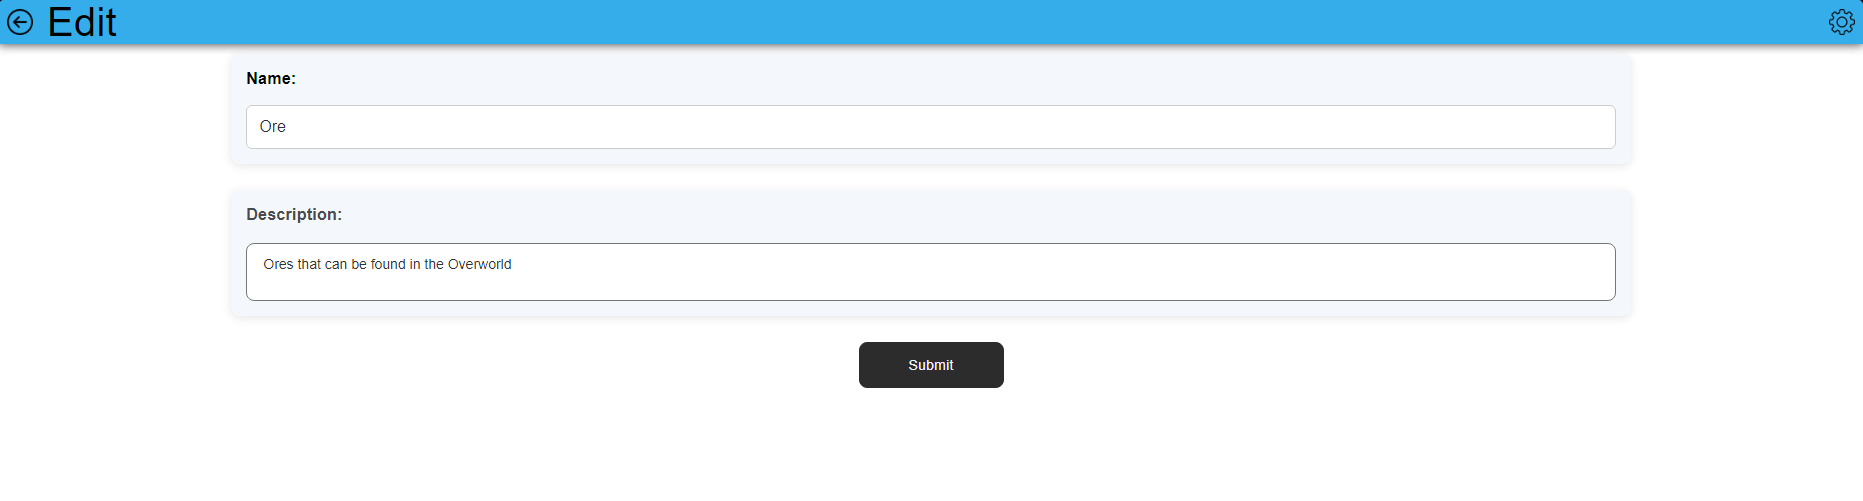
\includegraphics[width=\getImageWidth]{images/app-desktop/app-categories-edit-desktop.png}
                \caption{Widok edycji kategorii}
                \label{fig:app-categories-edit-desktop}
            \end{figure}

            \begin{figure}[H]
                \centering
                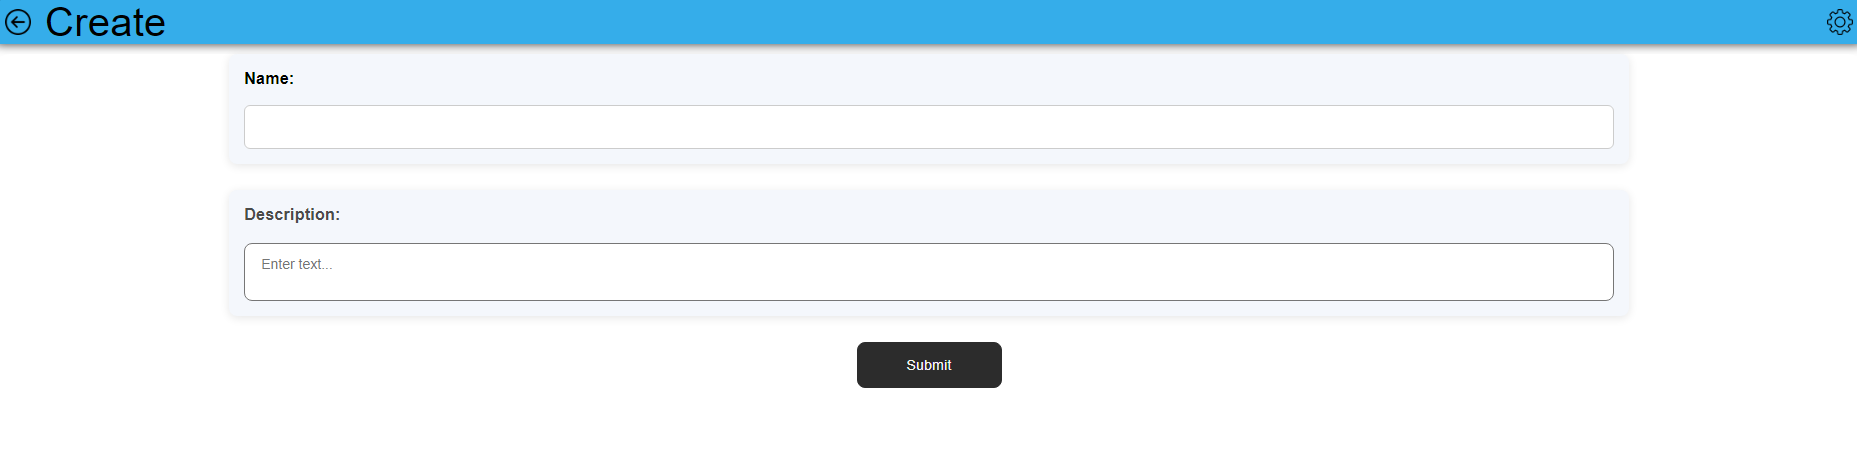
\includegraphics[width=\getImageWidth]{images/app-desktop/app-categories-add-desktop.png}
                \caption{Widok dodawania kategorii}
                \label{fig:app-categories-add-desktop}
            \end{figure}
        
        \FloatBarrier 
        \subsubsection{Magazyny}
            Strona magazynów przedstawiona na rysunku \ref{fig:app-warehouses-desktop} pozwala na przegląd i dodawanie magazynów. Podobnie jak w przypadku artykułów i kategorii w pasku górnym znajdują się te same opcje. Także analogicznie do artykułów i kategorii wybór magazynów następuje poprzez nacisnięcie odpowiedniego elementu. Dodatkowo na każdym wpisie znajduje się przycik, który przekierowuje do stanu danego magazynu.

            Widok szczegółow, edycji i dodawania nowej kategorii działa tak samo jak w przypadku artykułów i kategorii z dodatkiem interaktywnej mapy. Podczas wyświetlania szczegółów (Rysunek \ref{fig:app-warehouses-details-desktop}), mapa przedstawia wybraną lokalizację magazynu. Dodatkowo widok szczegółów zawiera przycisk, który przekierowuje bezpośrednio do stanu danego magazynu.

            \begin{figure}[H]
                \centering
                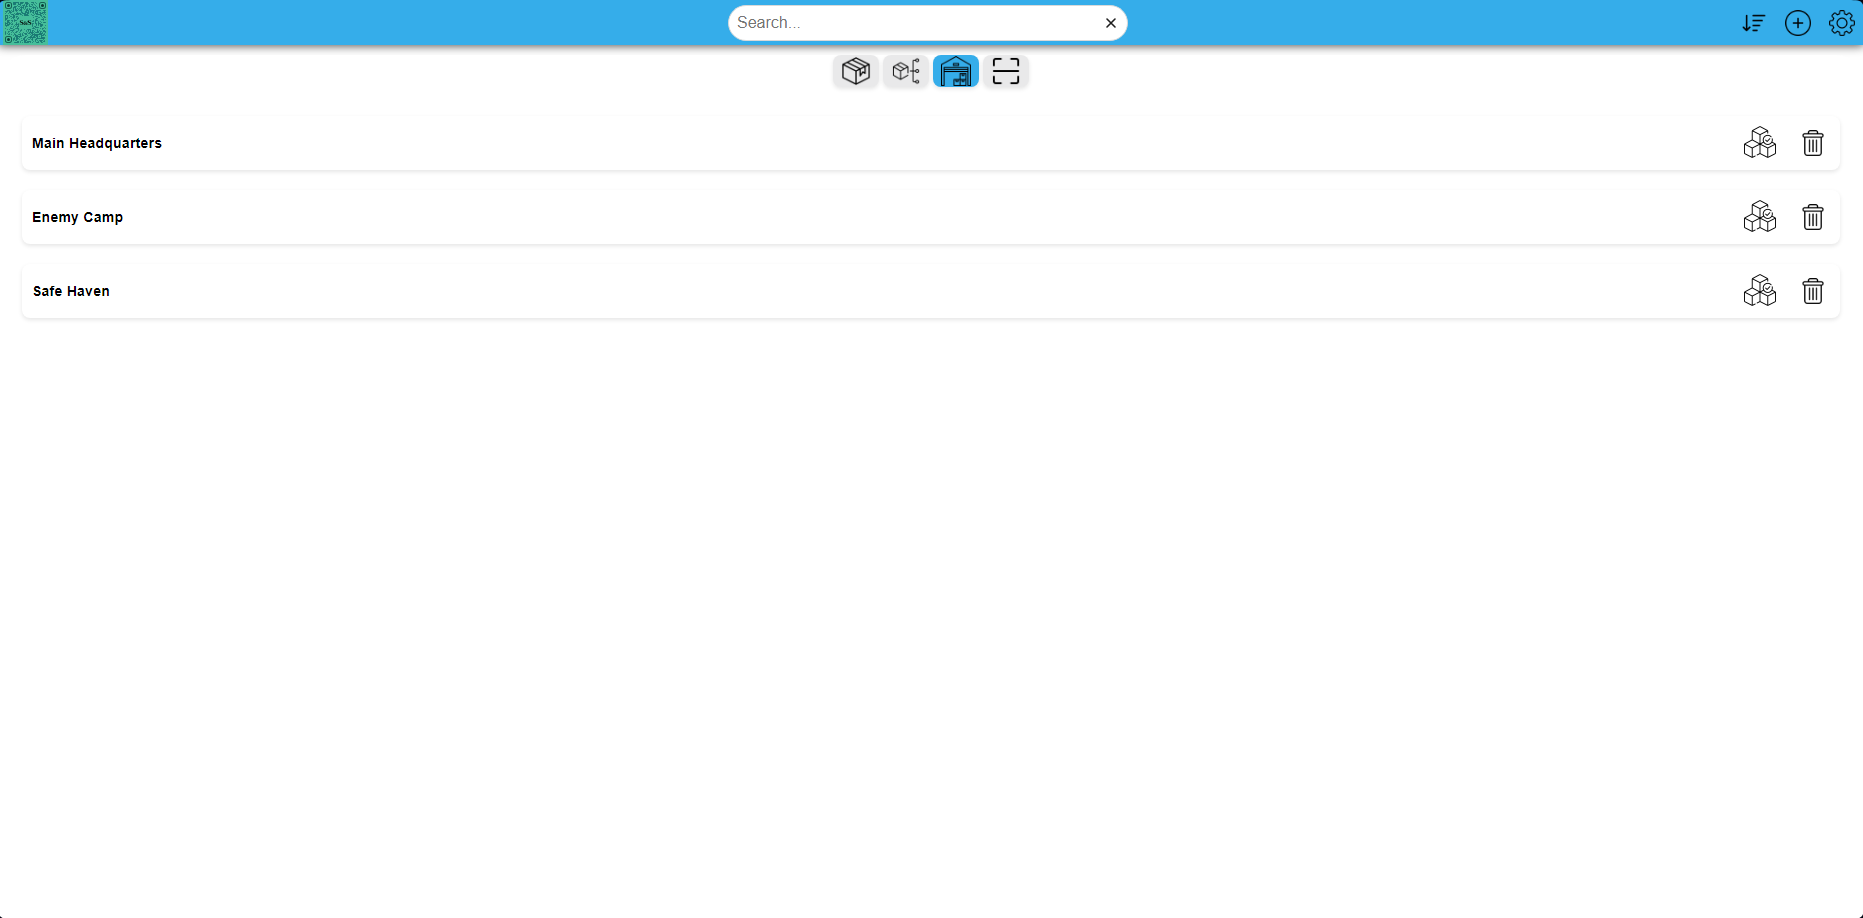
\includegraphics[width=\getImageWidth]{images/app-desktop/app-warehouses-desktop.png}
                \caption{Widok magazynów na komputerze stacjonarnym}
                \label{fig:app-warehouses-desktop}
            \end{figure}
                
            \begin{figure}[H]
                \centering
                
\includegraphics[height=\getImageHeight]{images/app-mobile/app-warehouses-mobile.png}
                \caption{Widok magazynów na telefonie komórkowym}
                \label{fig:app-warehouses-mobile}
            \end{figure}

            \begin{figure}[H]
                \begin{subfigure}{.49\textwidth}
                    \centering
                    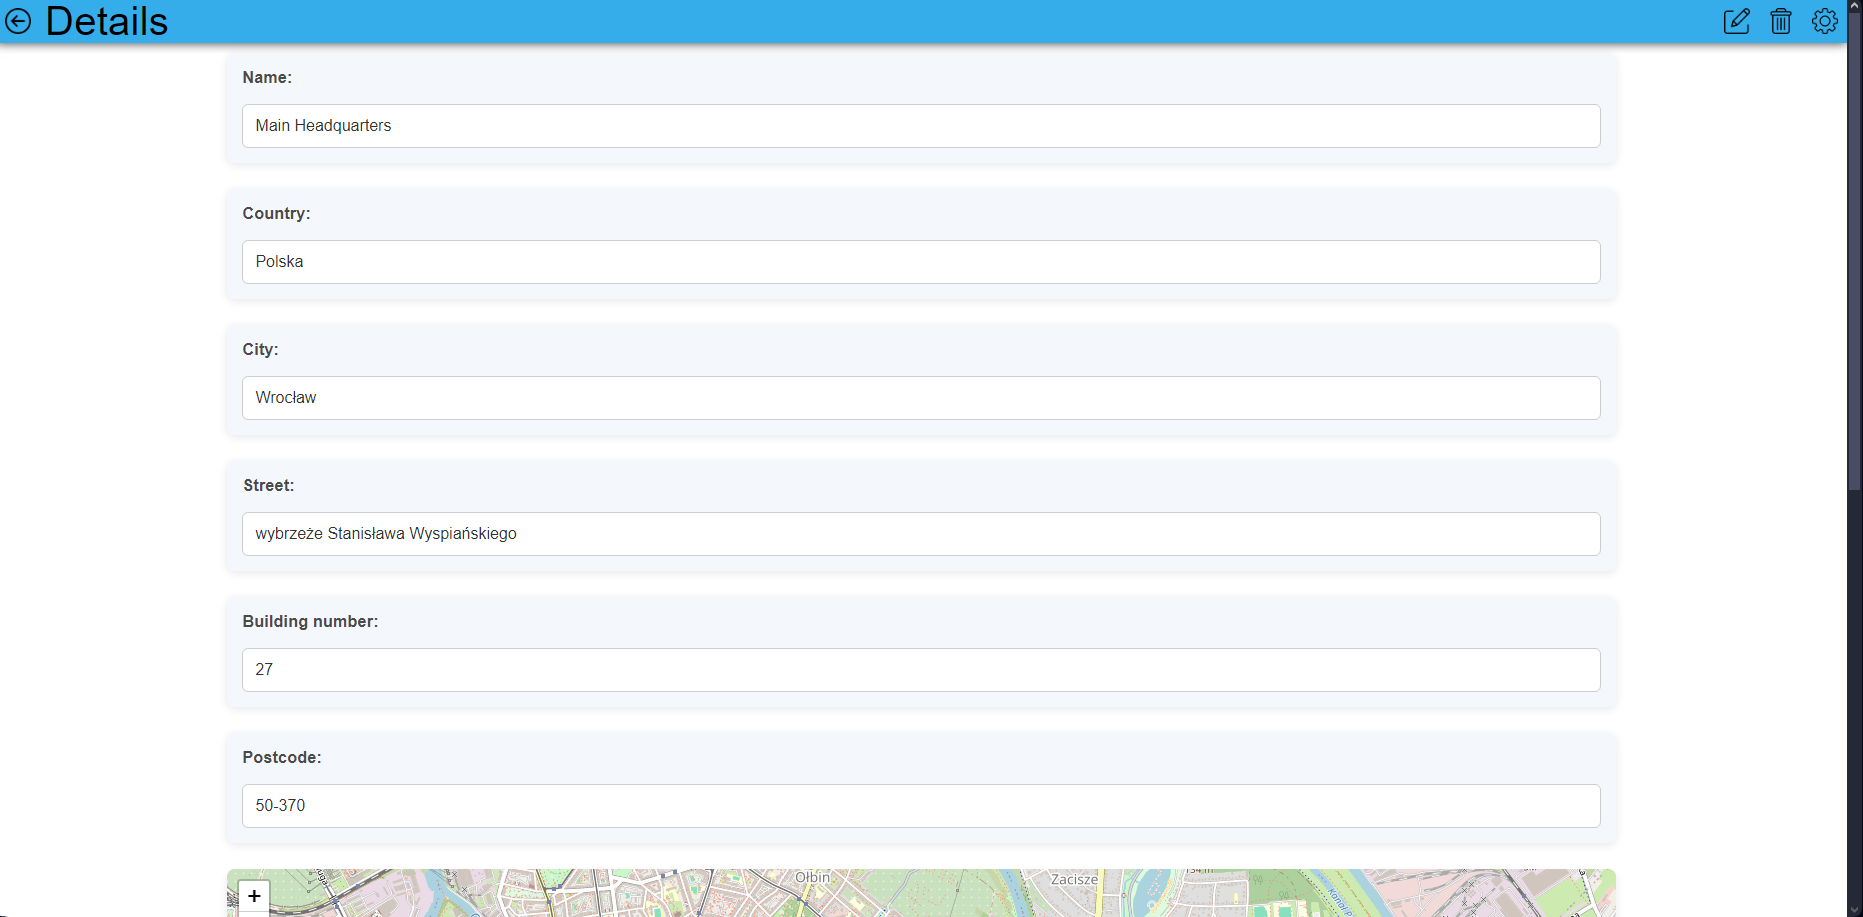
\includegraphics[width=\getImageWidth]{images/app-desktop/app-warehouses-details1-desktop.png}
                    \label{fig:app-warehouses-details1-desktop}
                \end{subfigure}
                \begin{subfigure}{.49\textwidth}
                    \centering
                    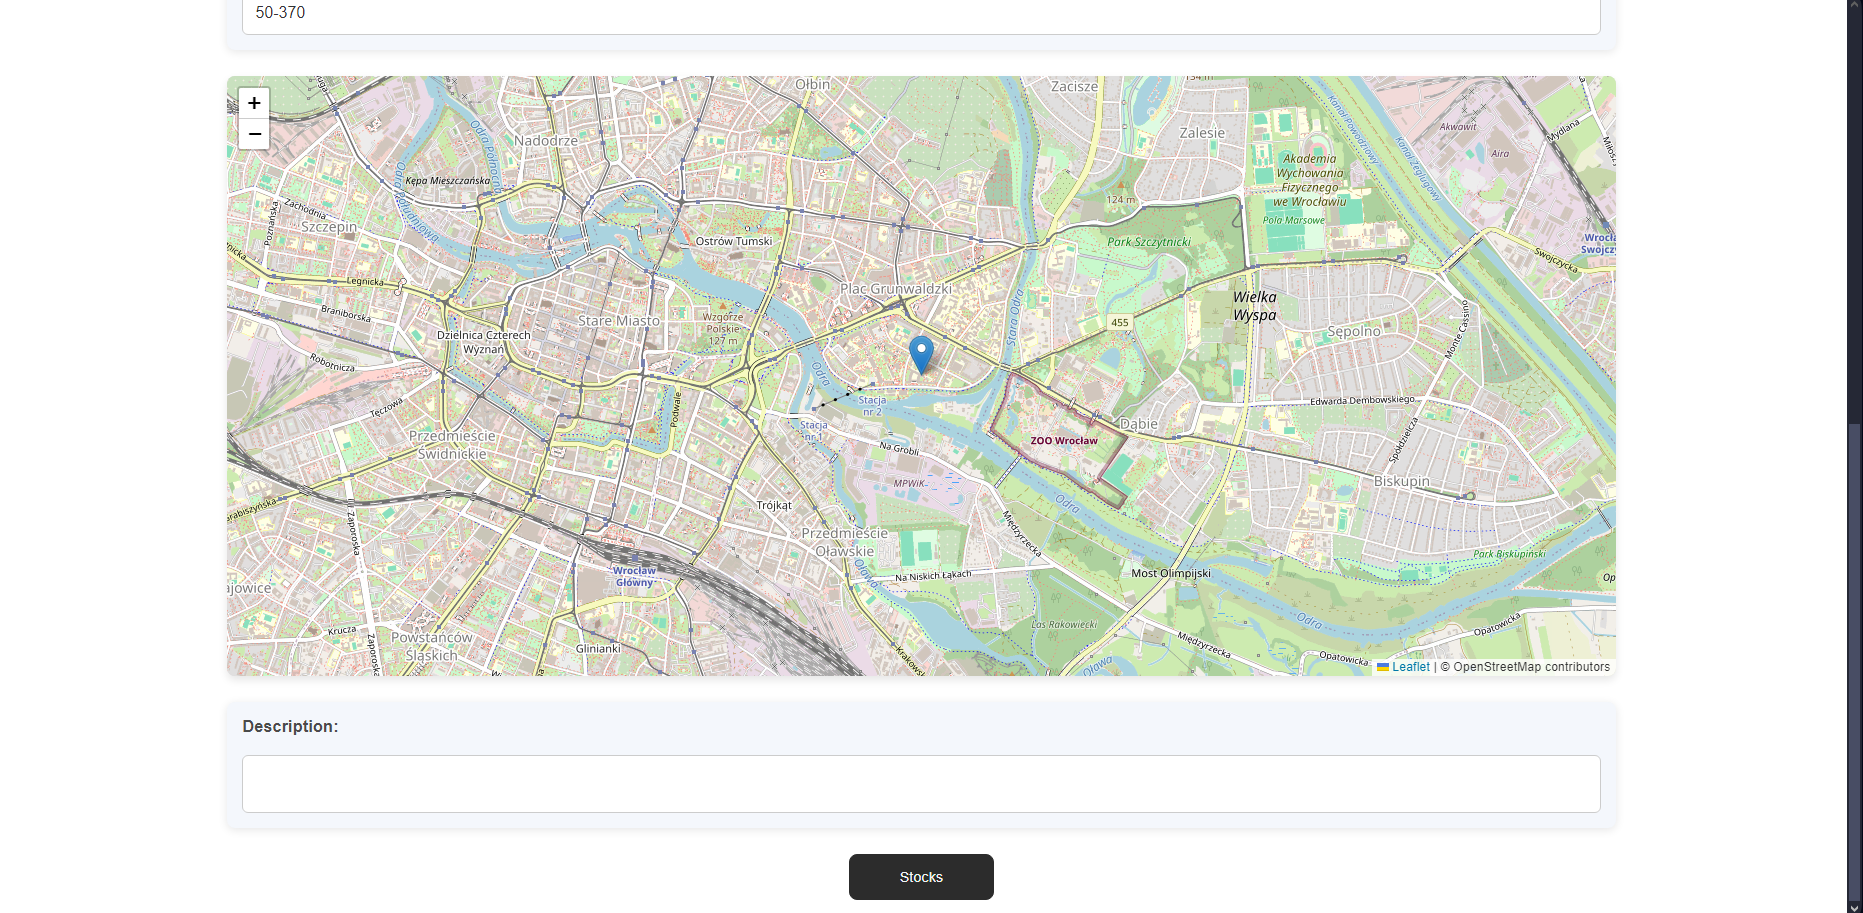
\includegraphics[width=\getImageWidth]{images/app-desktop/app-warehouses-details2-desktop.png}
                    \label{fig:app-warehouses-details2-desktop}
                \end{subfigure}
                \caption{Widok szczegółow magazynu}
                \label{fig:app-warehouses-details-desktop}
            \end{figure}
            
            Podczas edycji (Rysunek \ref{fig:app-warehouses-edit-desktop}), mapa jest interaktywna i pozwala na wybór lokalizacji poprzez przeniesienie pinezki w wybrane miejsce. Wszystkie pola, które mogą być wypełnione, zostaną automatycznie zaktualizowane. Podobnie w przypadku wprowadzenia nowego adresu mapa zaktualizuję się aby odzwierciedlić zmiany.

            \begin{figure}[H]
                \begin{subfigure}{.49\textwidth}
                    \centering
                    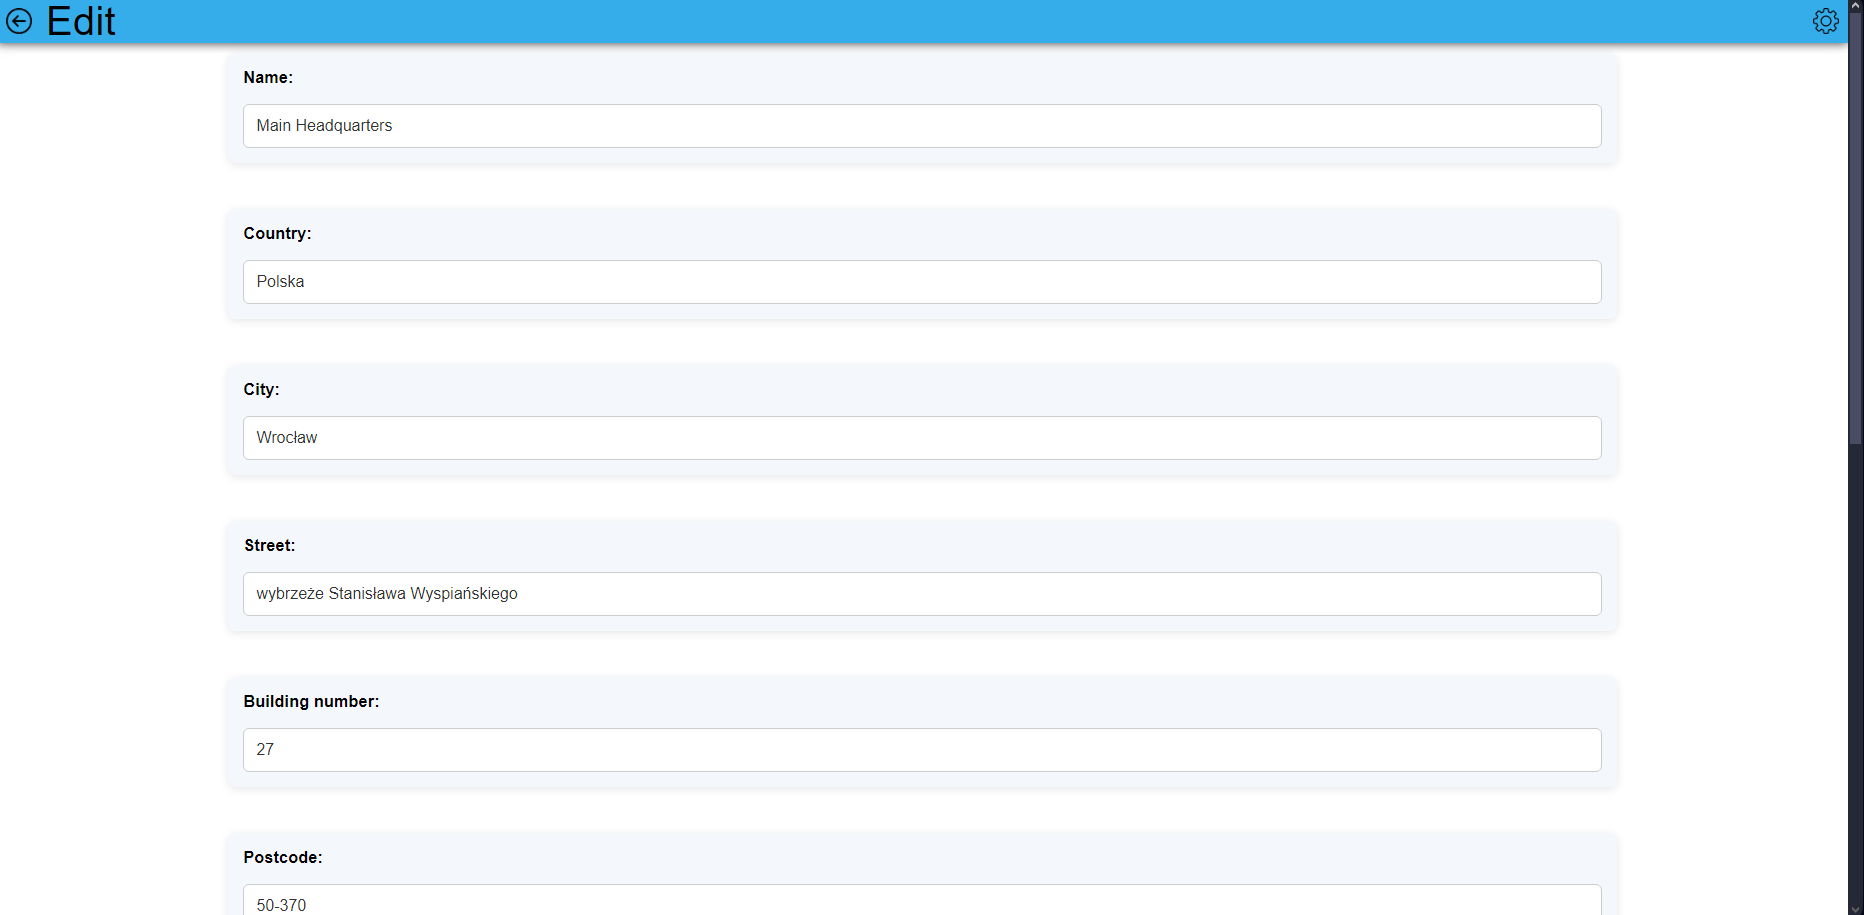
\includegraphics[width=\getImageWidth]{images/app-desktop/app-warehouses-edit1-desktop.png}
                    \label{fig:app-warehouses-edit1-desktop}
                \end{subfigure}
                \begin{subfigure}{.49\textwidth}
                    \centering
                    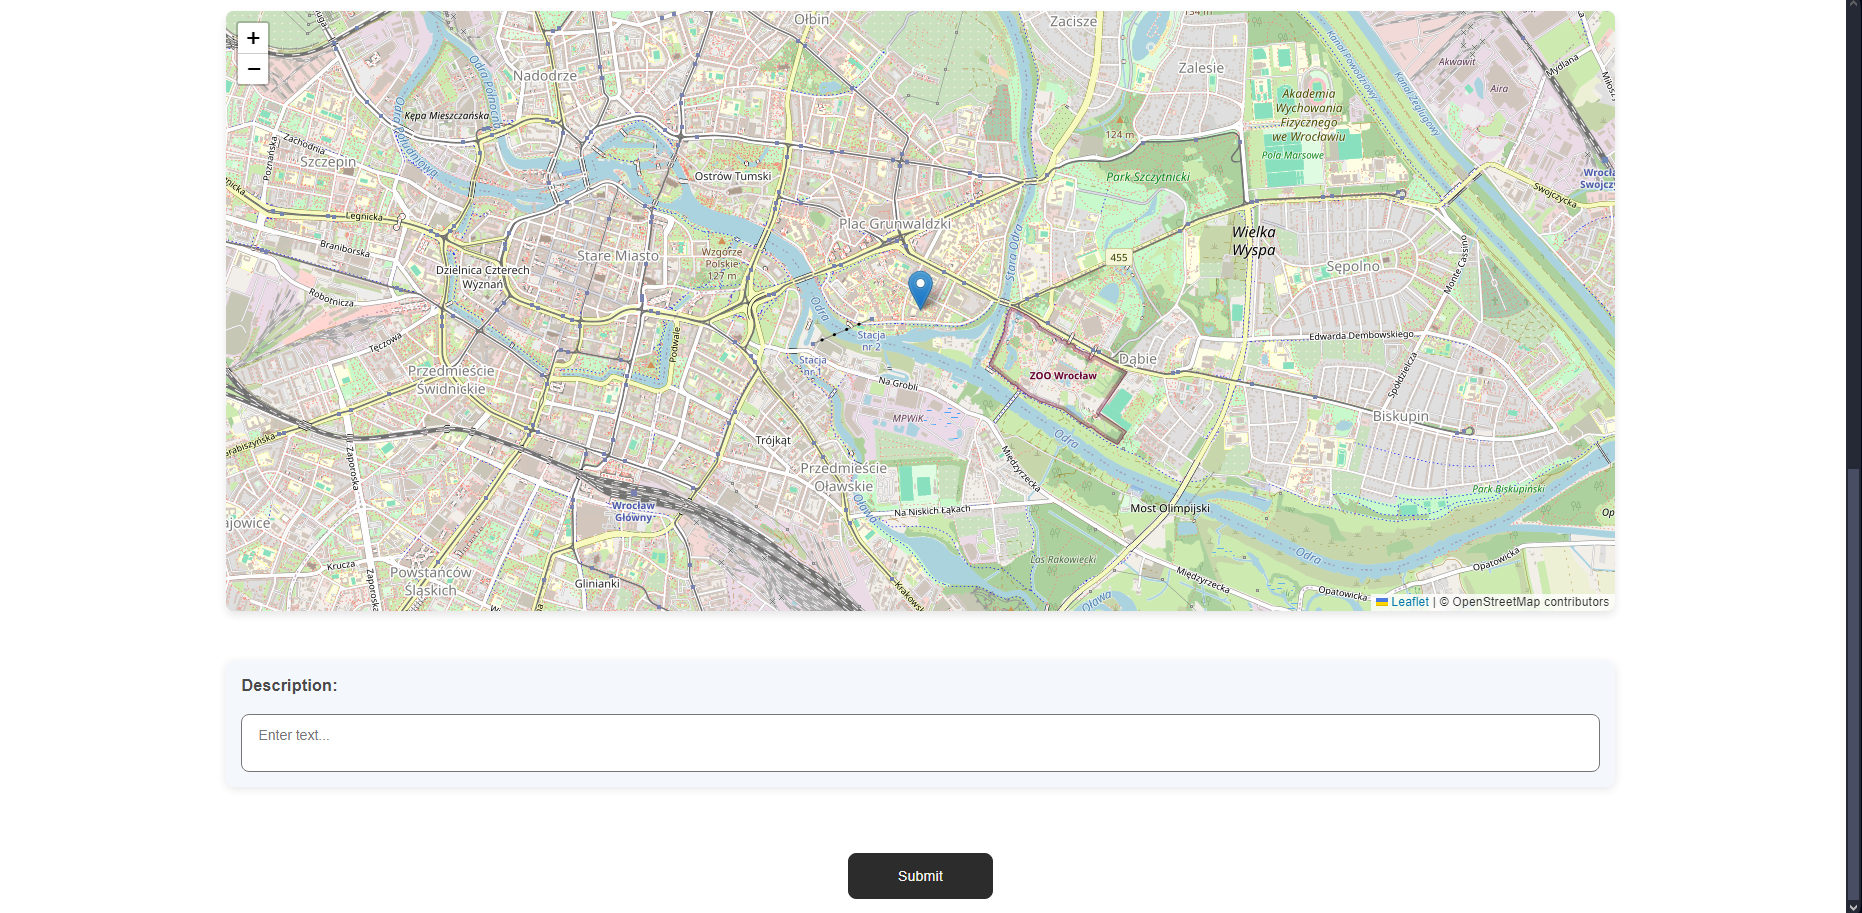
\includegraphics[width=\getImageWidth]{images/app-desktop/app-warehouses-edit2-desktop.png}
                    \label{fig:app-warehouses-edit2-desktop}
                \end{subfigure}
                \caption{Widok edycji magazynu}
                \label{fig:app-warehouses-edit-desktop}
            \end{figure}

            Podobnie jak w przypadku edycji, podczas dodawania nowego magazynu (Rysunek \ref{fig:app-warehouses-add-desktop}) mapa jest interaktywna i zachowuje się w ten sam sposób.

            \begin{figure}[H]
                \begin{subfigure}{.49\textwidth}
                    \centering
                    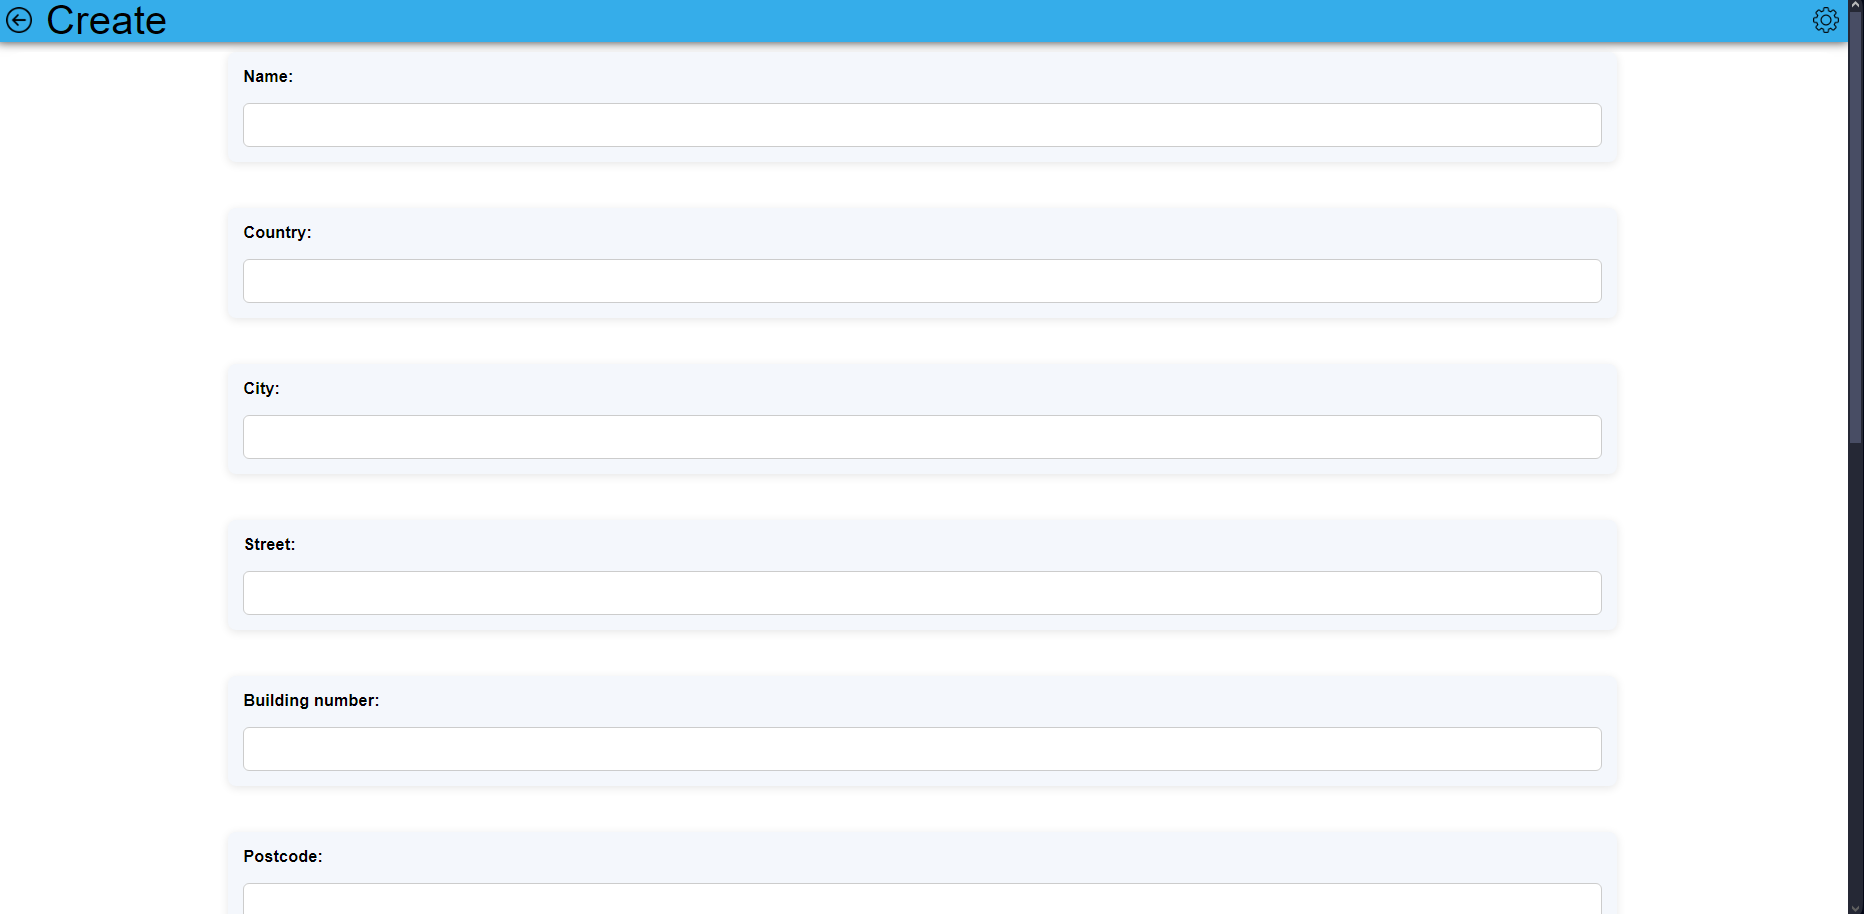
\includegraphics[width=\getImageWidth]{images/app-desktop/app-warehouses-add1-desktop.png}
                    \label{fig:app-warehouses-add1-desktop}
                \end{subfigure}
                \begin{subfigure}{.49\textwidth}
                    \centering
                    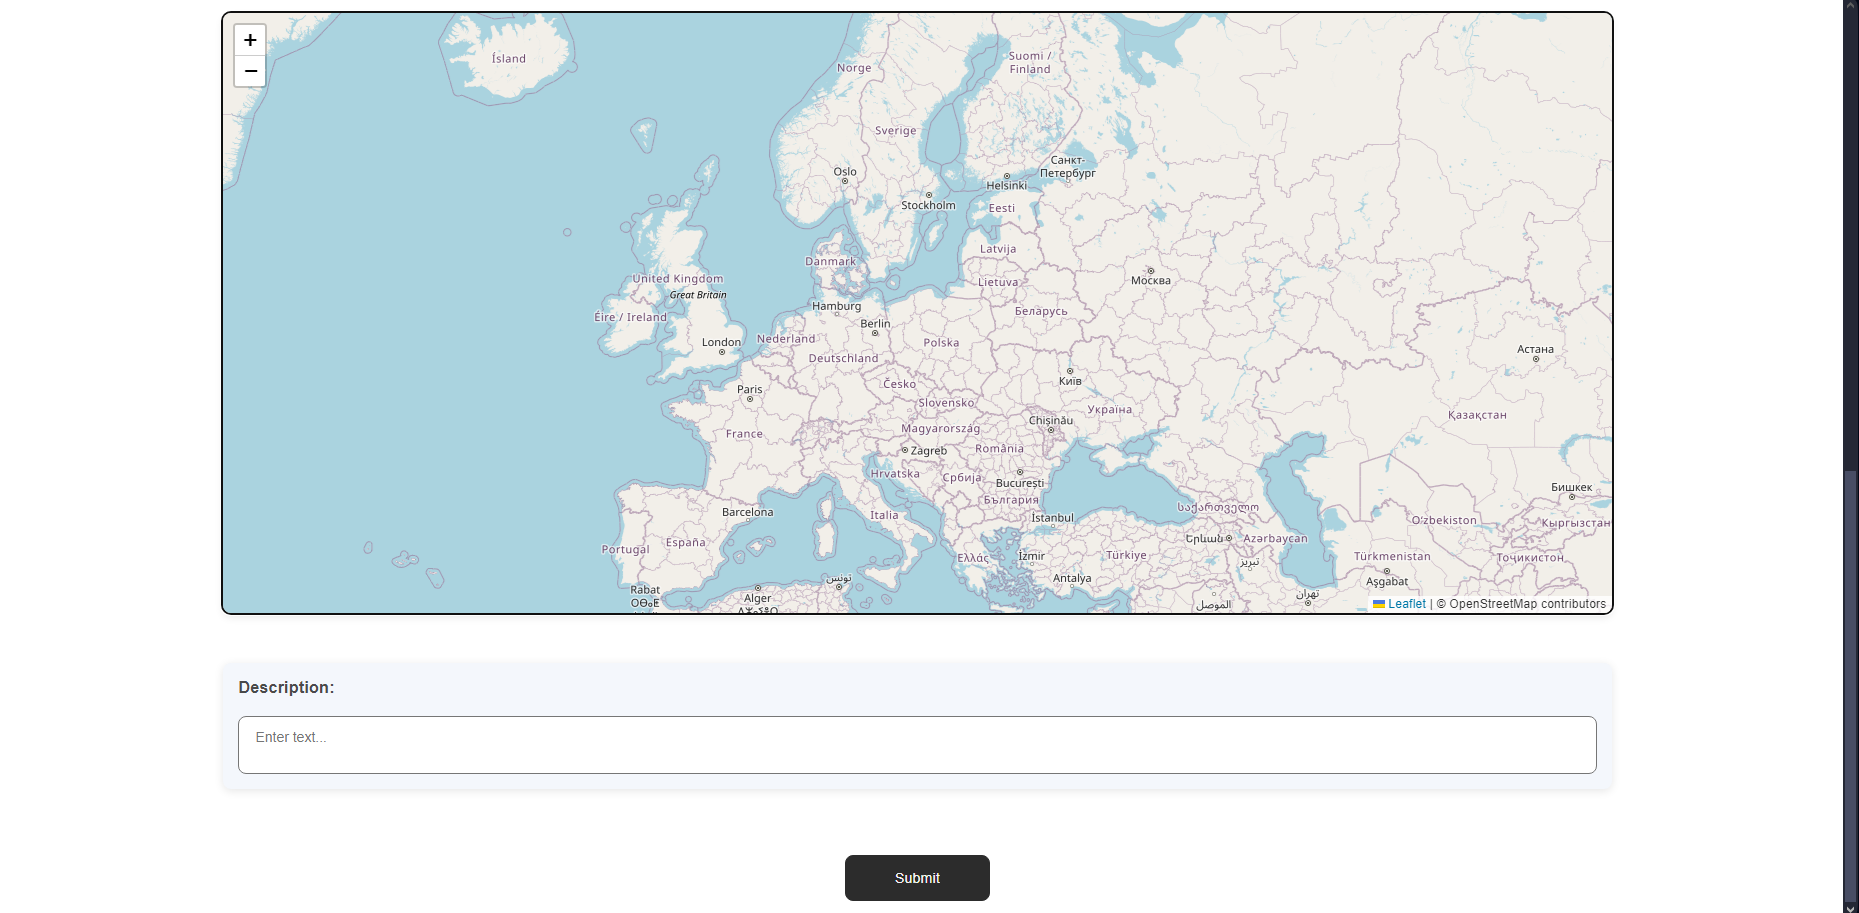
\includegraphics[width=\getImageWidth]{images/app-desktop/app-warehouses-add2-desktop.png}
                    \label{fig:app-warehouses-add2-desktop}
                \end{subfigure}
                \caption{Widok dodawania magazynu}
                \label{fig:app-warehouses-add-desktop}
            \end{figure}

        \FloatBarrier 
        \subsubsection{Ustawienia}
            Widok ustawień (Rysunek \ref{fig:app-settings-desktop}) oferuje 3 funkcjonalności: ustalenie domyślnego magazynu, wylogowanie się z aplikacji oraz odświeżenie obrazków na wypadek jakichkolwiek problemów z funkcją cache.
            Przycisk wylogowania przekierowuje użytkownika na strone startową i go wylogowuje. Odświeżenie obrazków powoduje wyczyszczenie wszystkich zapamiętanych obrazków i pozwala na ponowne pobranie ich z serwera.
            
            Selekcja domyślnego magazynu przebiega poprzez wybranie jednego ze stworzonych wcześniej magazynu z listy, lub kliknięcie w odpowiednią pinezkę na mapie.

            Po ustaleniu domyślnego magazynu w głównych widokach pojawi się nowa ikona oznaczająca stan domyślnego magazynu co przedstawia Rysunek \ref{fig:app-warehouses-with-default-desktop}.

            \begin{figure}[H]
                \centering
                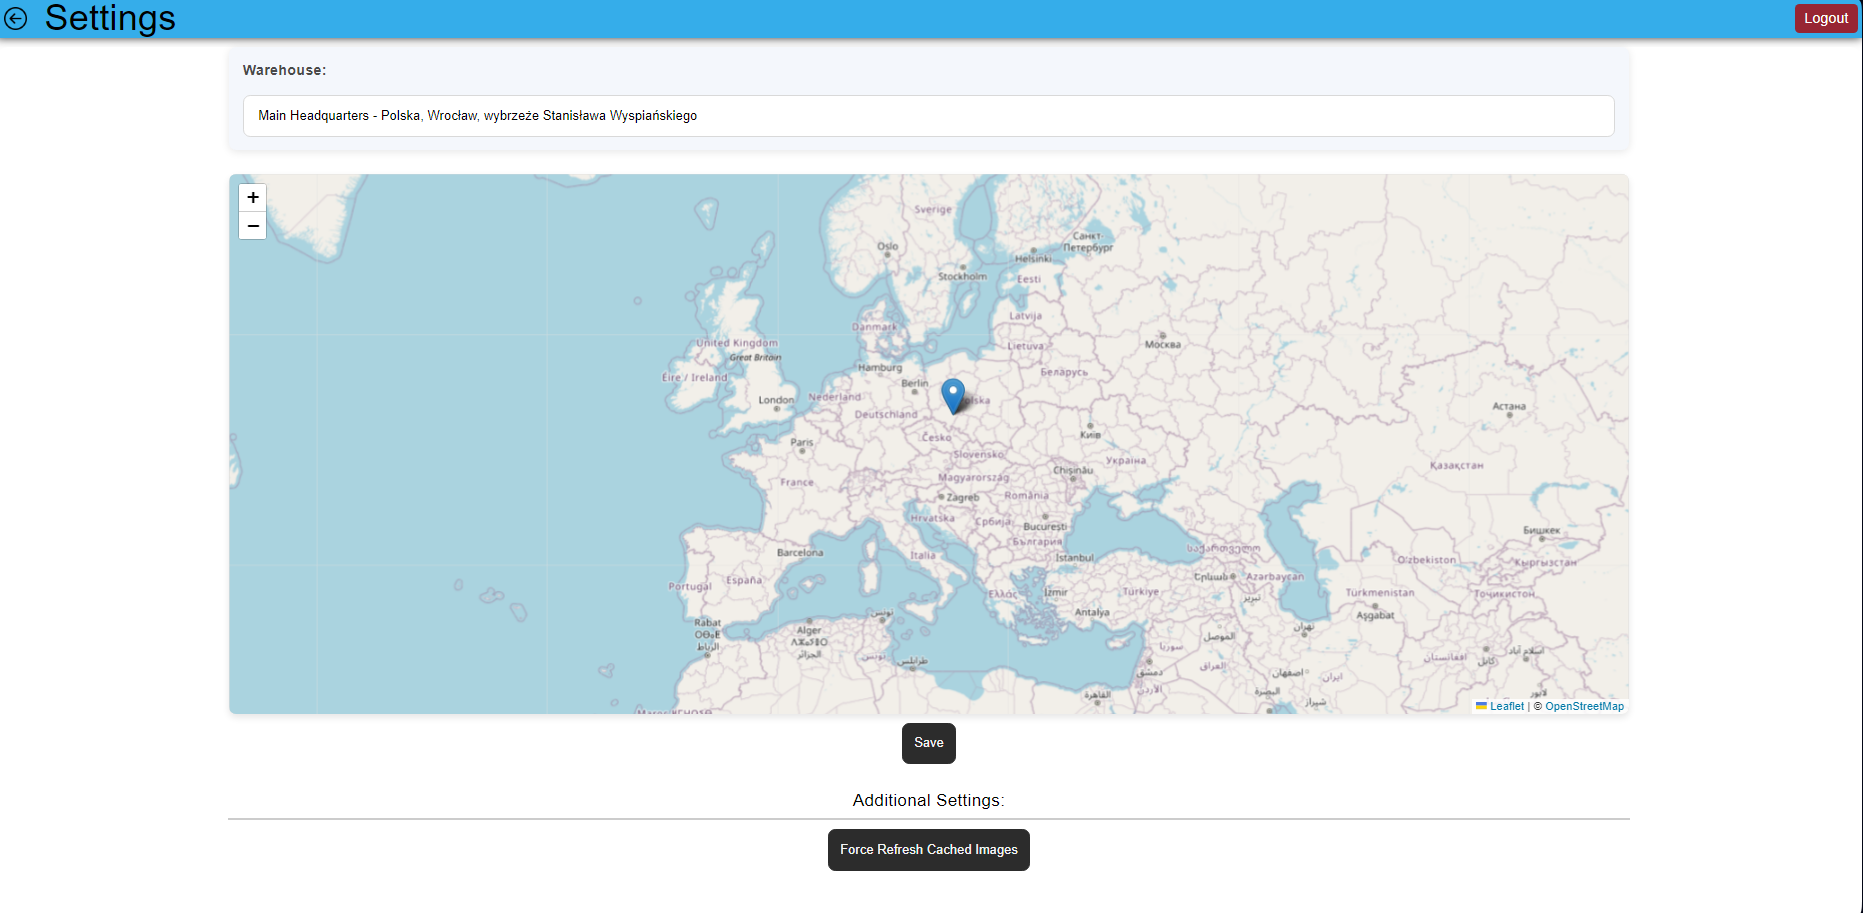
\includegraphics[width=\getImageWidth]{images/app-desktop/app-settings-desktop.png}
                \caption{Widok ustawień na komputerze stacjonarnym}
                \label{fig:app-settings-desktop}
            \end{figure}
            
            \begin{figure}[H]
                \centering
                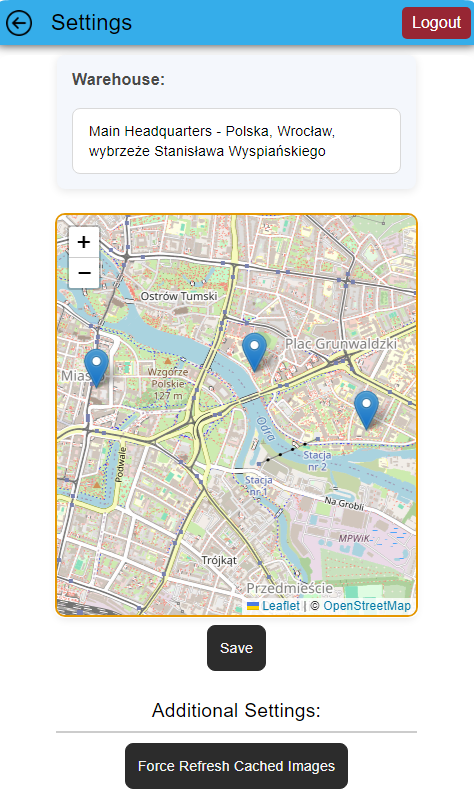
\includegraphics[height=\getImageHeight]{images/app-mobile/app-settings-mobile.png}
                \caption{Widok ustawień na telefonie komórkowym}
                \label{fig:app-settings-mobile}
            \end{figure}

            \begin{figure}[H]
                \centering
                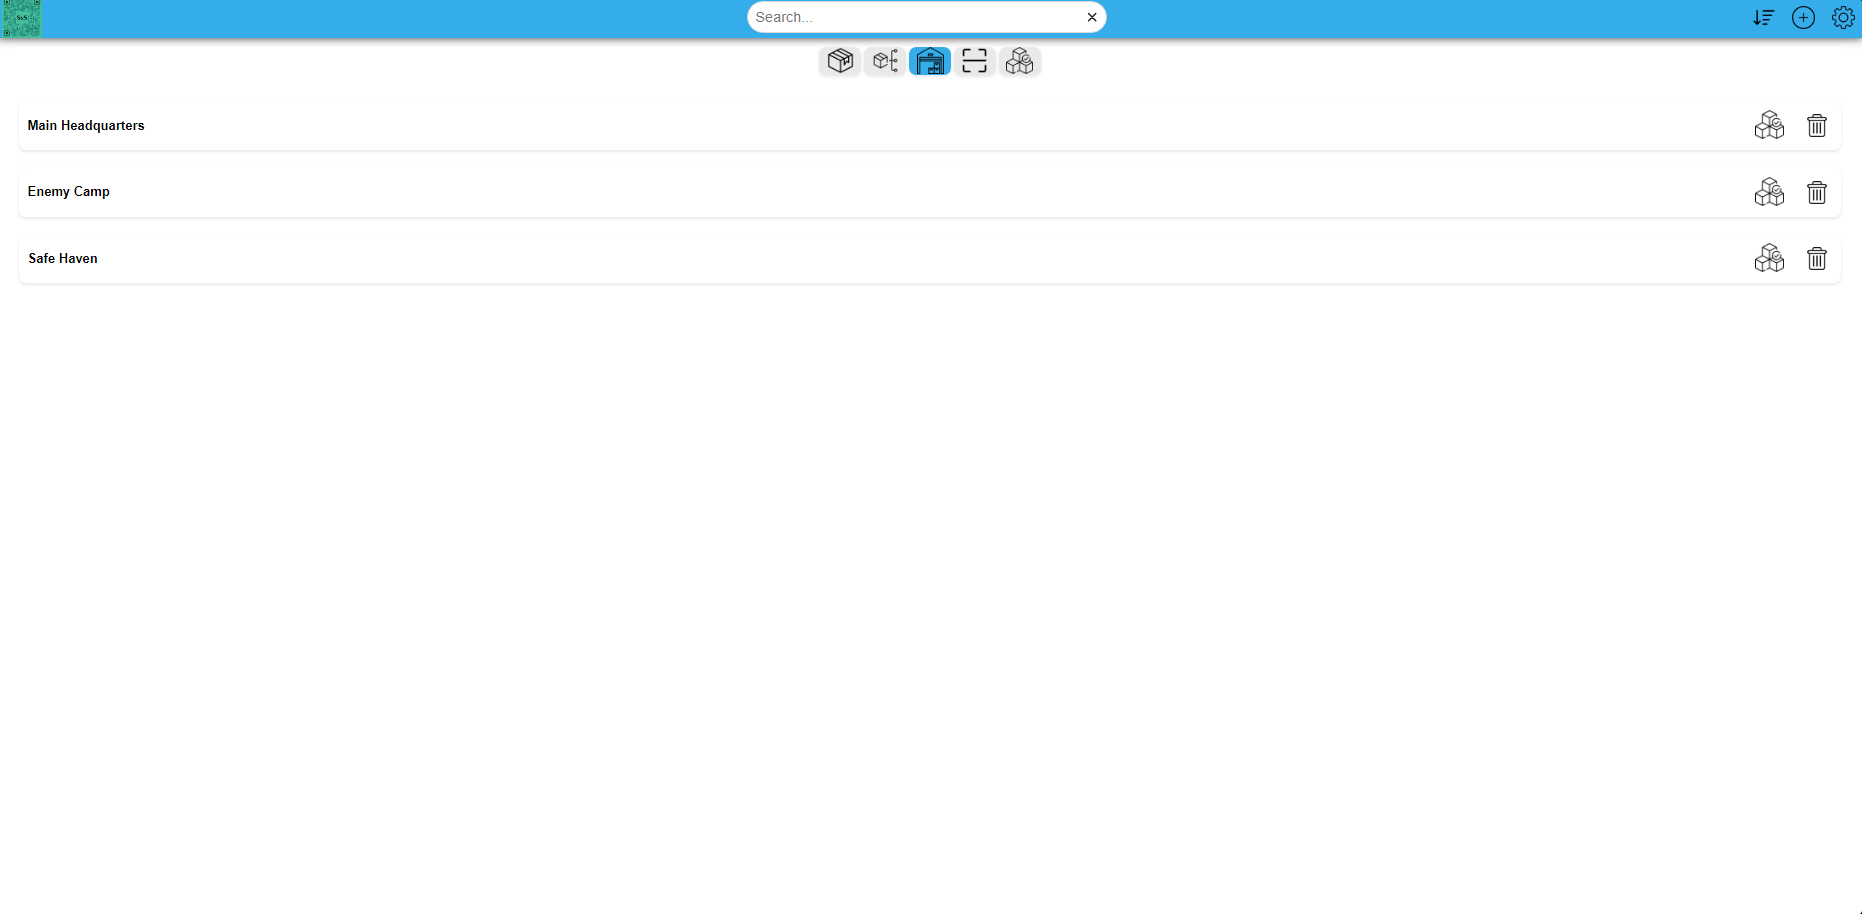
\includegraphics[width=\getImageWidth]{images/app-desktop/app-warehouses-with-default-desktop.png}
                \caption{Widok magazynów po ustaleniu domyślnego magazynu}
                \label{fig:app-warehouses-with-default-desktop}
            \end{figure}

        \FloatBarrier 
        \subsubsection{Stan magazynu}
            Widok stanu magazynu ma dwie postaci: dowolny magazyn (Rysunek \ref{fig:app-stock-any-desktop}) oraz magazyn domyślny (Rysunek \ref{fig:app-stock-default-desktop}), gdzie jedyną różnicą jest podświetlenie ikony domyślnego magazynu. Funkcje górnego paska są takie same jak w widoku artykułu, z tą róznicą, że przycisk dodawania pozwala na wprowadzenie nowego przedmiotu na stan magazynu. W widoku szczegółow (Rysunek \ref{fig:app-stock-details-desktop}) wyświetlane są informacje o przedmiocie, takie jak obrazek, nazwa, kategoria, opis i kod EAN13, nazwa aktualnego magazynu minimalna liczba sztuk oraz aktualna liczba sztuk danego przedmiotu. Minimalna liczba sztuk jest określana w celu zawiadamiania odpowiednich użytkowników w momencie kiedy stan danego przedmiotu w magazynie spadnie poniżej wymaganej wartości.

            \begin{figure}[H]
                \centering
                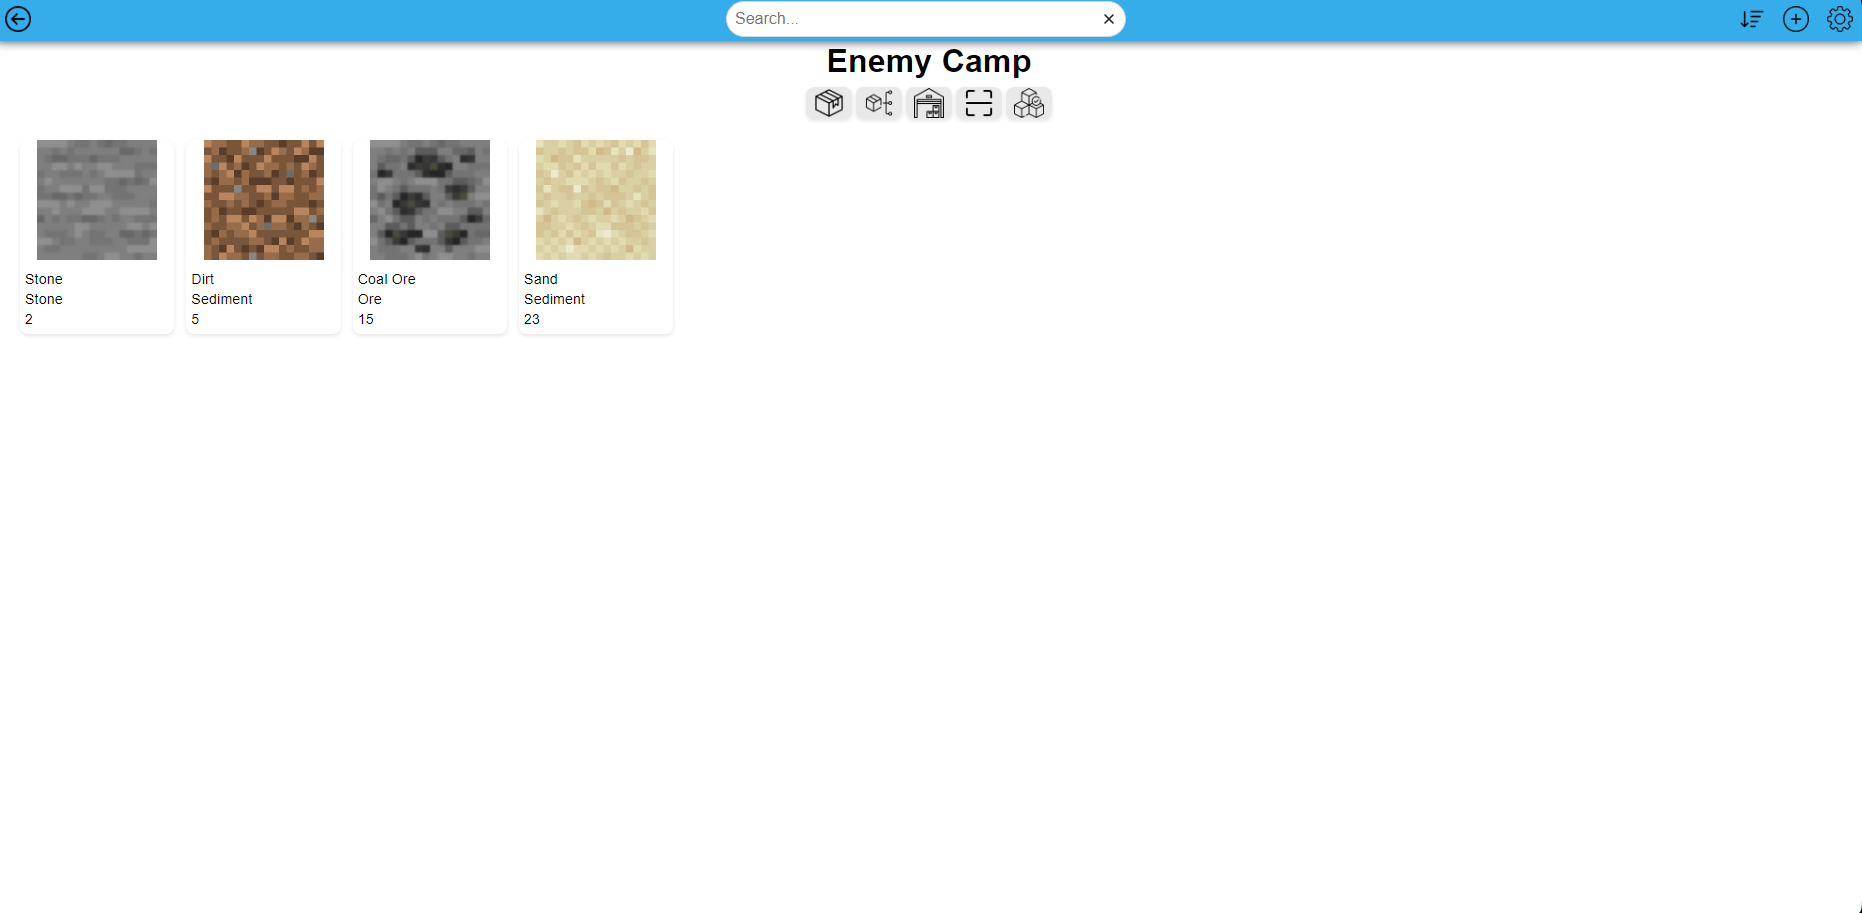
\includegraphics[width=\getImageWidth]{images/app-desktop/app-stock-any-desktop.png}
                \caption{Widok stanu magazynu dla dowolnego magazynu na komputerze stacjonarnym}
                \label{fig:app-stock-any-desktop}
            \end{figure}
            \begin{figure}[H]
                \centering
                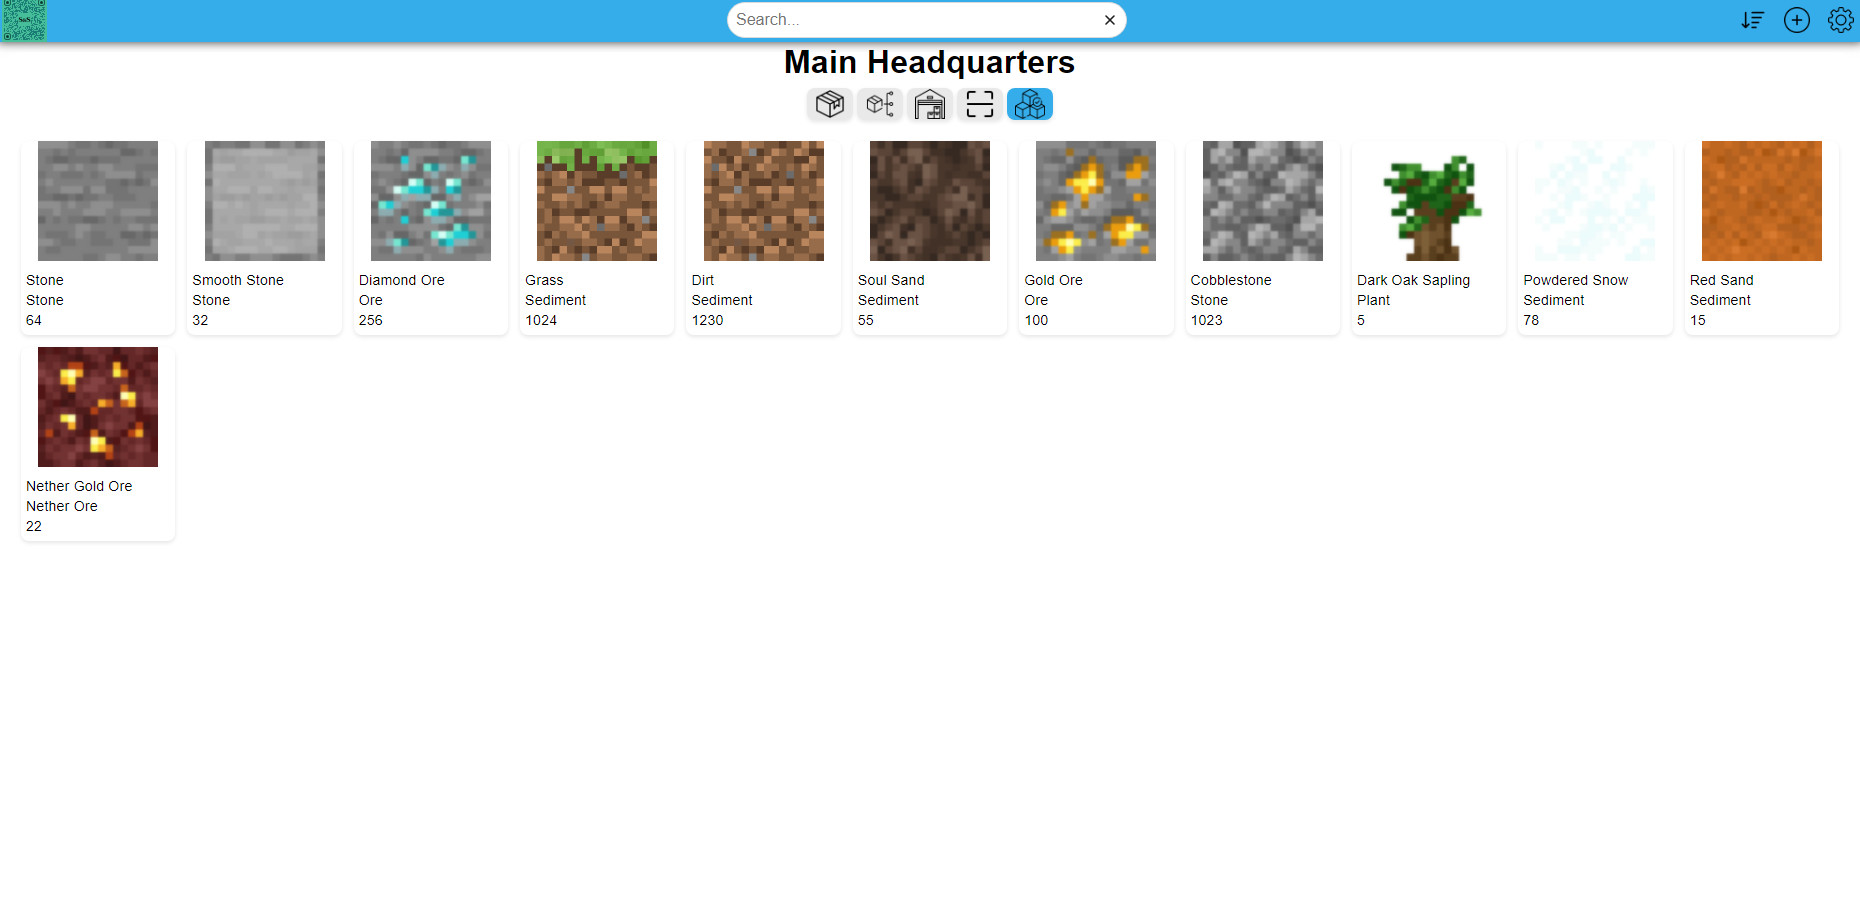
\includegraphics[width=\getImageWidth]{images/app-desktop/app-stock-default-desktop.png}
                \caption{Widok stanu magazynu dla domyślnego magazynu na komputerze stacjonarnym}
                \label{fig:app-stock-default-desktop}
            \end{figure}
            
            \begin{figure}[H]
                \centering
                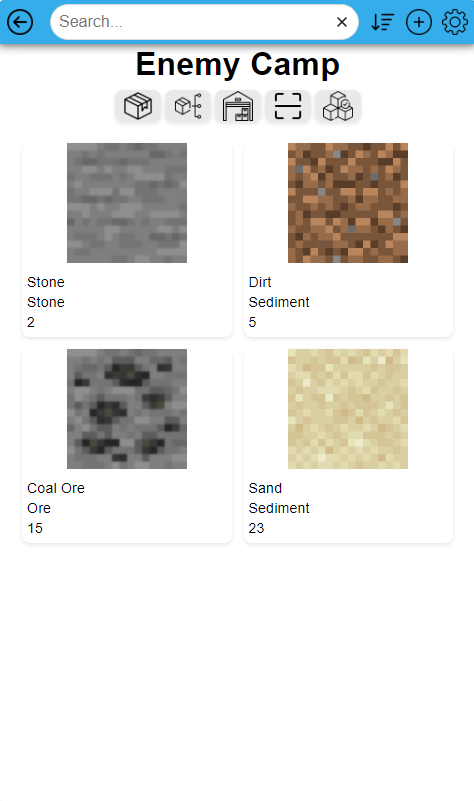
\includegraphics[height=\getImageHeight]{images/app-mobile/app-stock-any-mobile.png}
                \caption{Widok stanu magazynu dla dowolnego magazynu na telefonie komórkowym}
                \label{fig:app-stock-any-mobile}
            \end{figure}
            \begin{figure}[H]
                \centering
                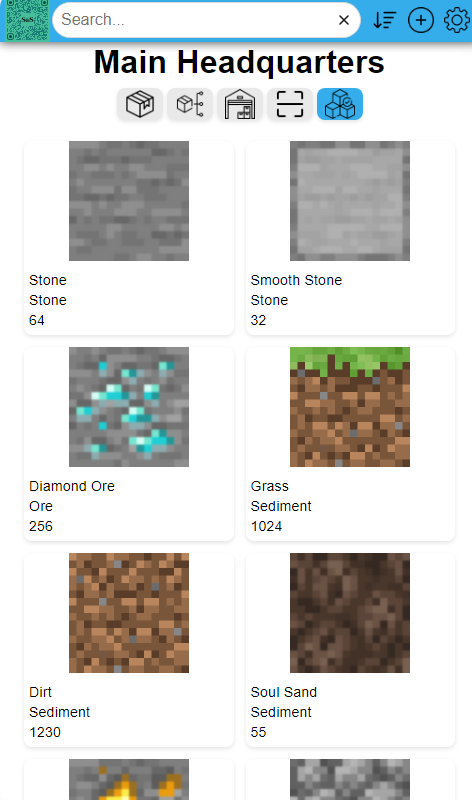
\includegraphics[height=\getImageHeight]{images/app-mobile/app-stock-default-mobile.png}
                \caption{Widok stanu magazynu dla domyślnego magazynu na telefonie komórkowym}
                \label{fig:app-stock-default-mobile}
            \end{figure}

            \begin{figure}[H]
                \begin{subfigure}{.49\textwidth}
                    \centering
                    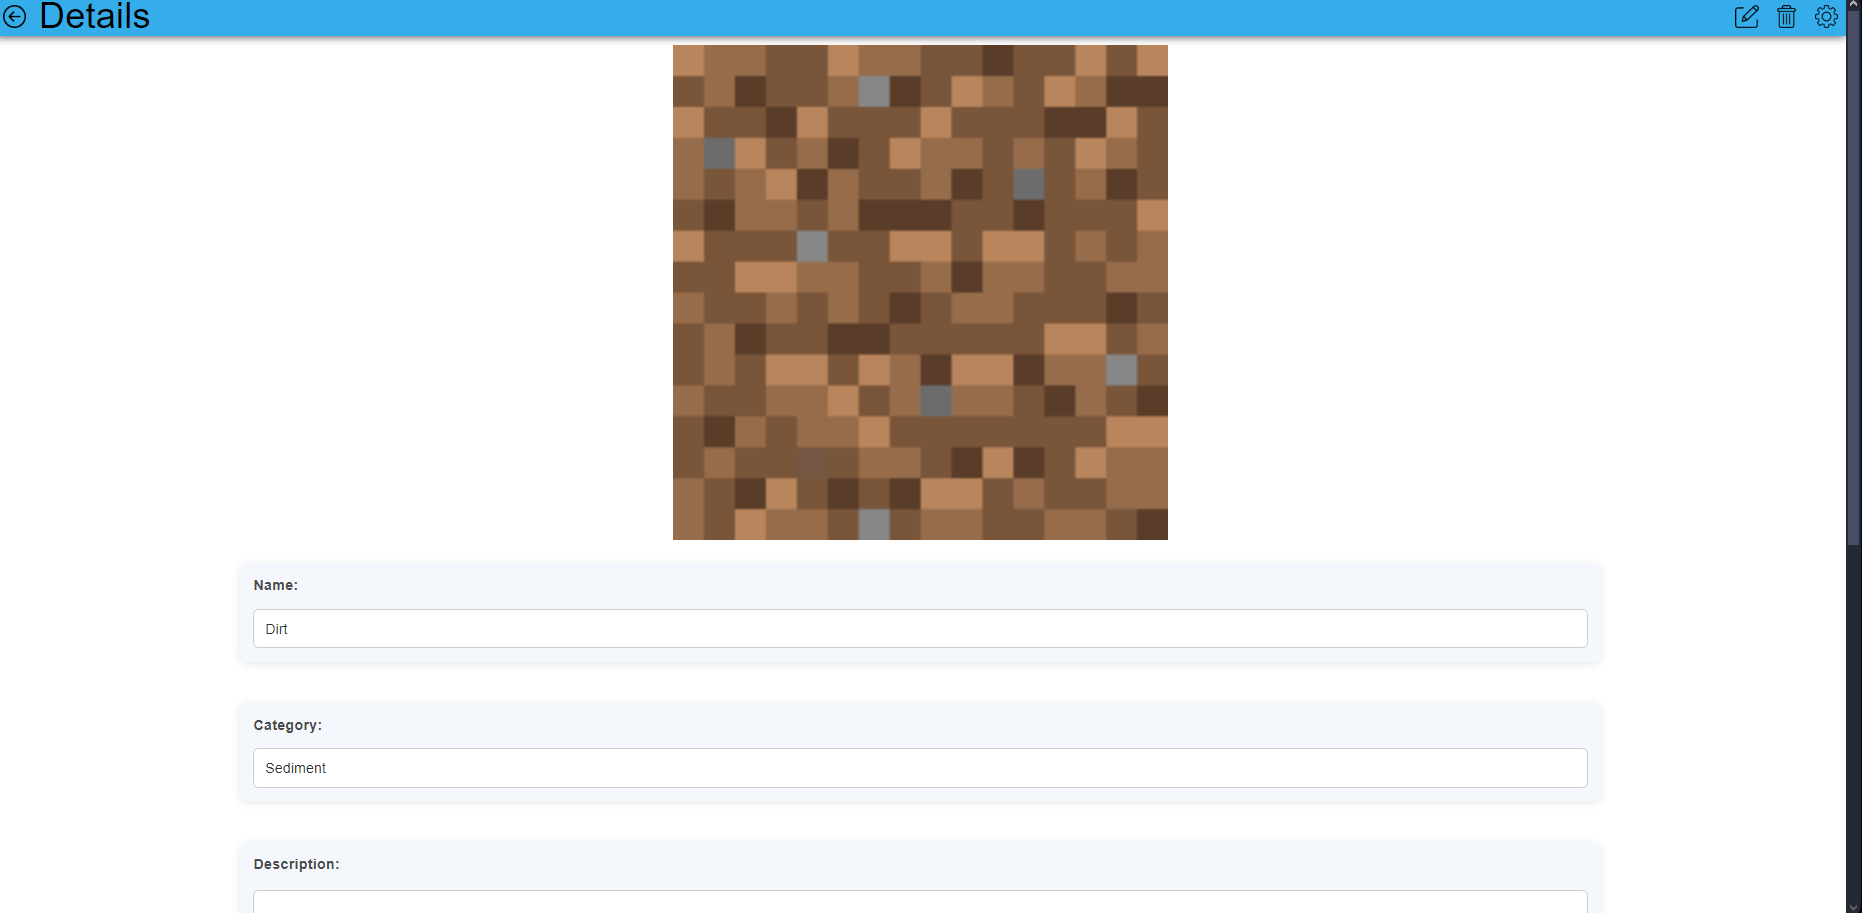
\includegraphics[width=\getImageWidth]{images/app-desktop/app-stock-details1-desktop.png}
                    \label{fig:app-stock-details1-desktop}
                \end{subfigure}
                \begin{subfigure}{.49\textwidth}
                    \centering
                    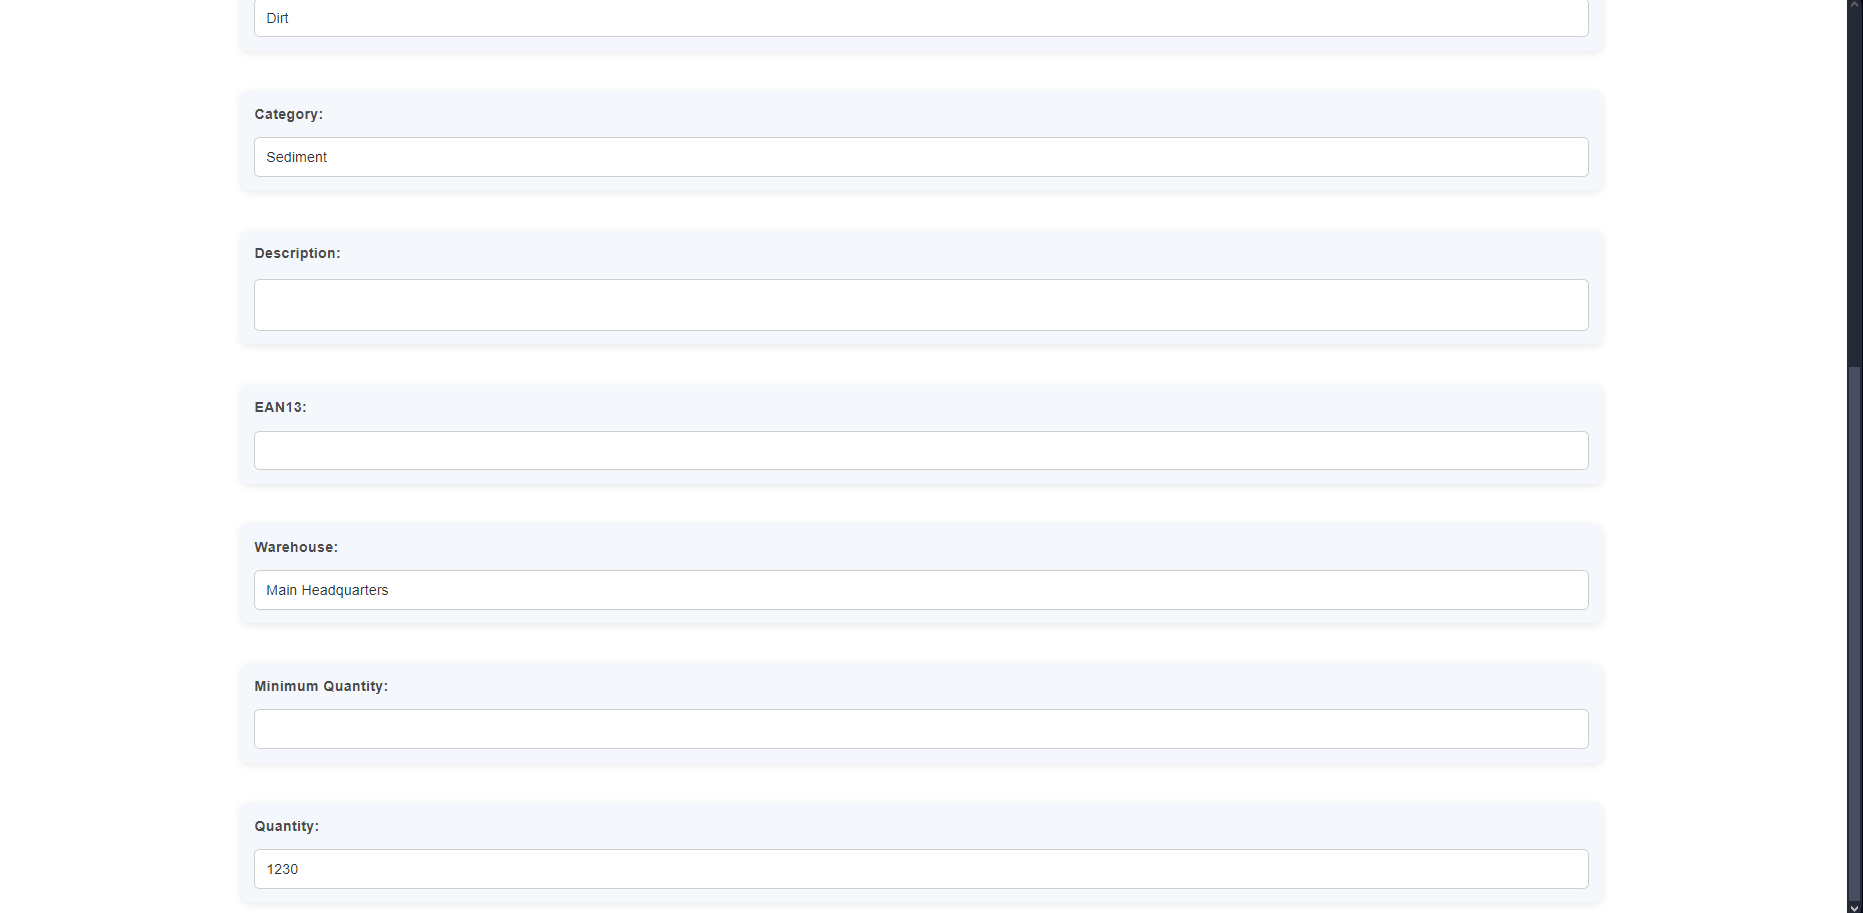
\includegraphics[width=\getImageWidth]{images/app-desktop/app-stock-details2-desktop.png}
                    \label{fig:app-stock-details2-desktop}
                \end{subfigure}
                \caption{Widok szczegółów stanu magazynu}
                \label{fig:app-stock-details-desktop}
            \end{figure}
            
            Edycja stanu magazynu przedstawiona na Rysunku \ref{fig:app-stock-edit-desktop} pozwala na określenie zmiany w liczbie sztuk danego przedmiotu. Zmiana może być dodatnia (wprowadzanie dodatkowych przedmiotów do magazynu) lub ujemna (wydawanie przedmiotów z magazynu). Zmiany można zatwierdzić lub anulować wybierając odpowiedni przycisk.

            \begin{figure}[H]
                \begin{subfigure}{.49\textwidth}
                    \centering
                    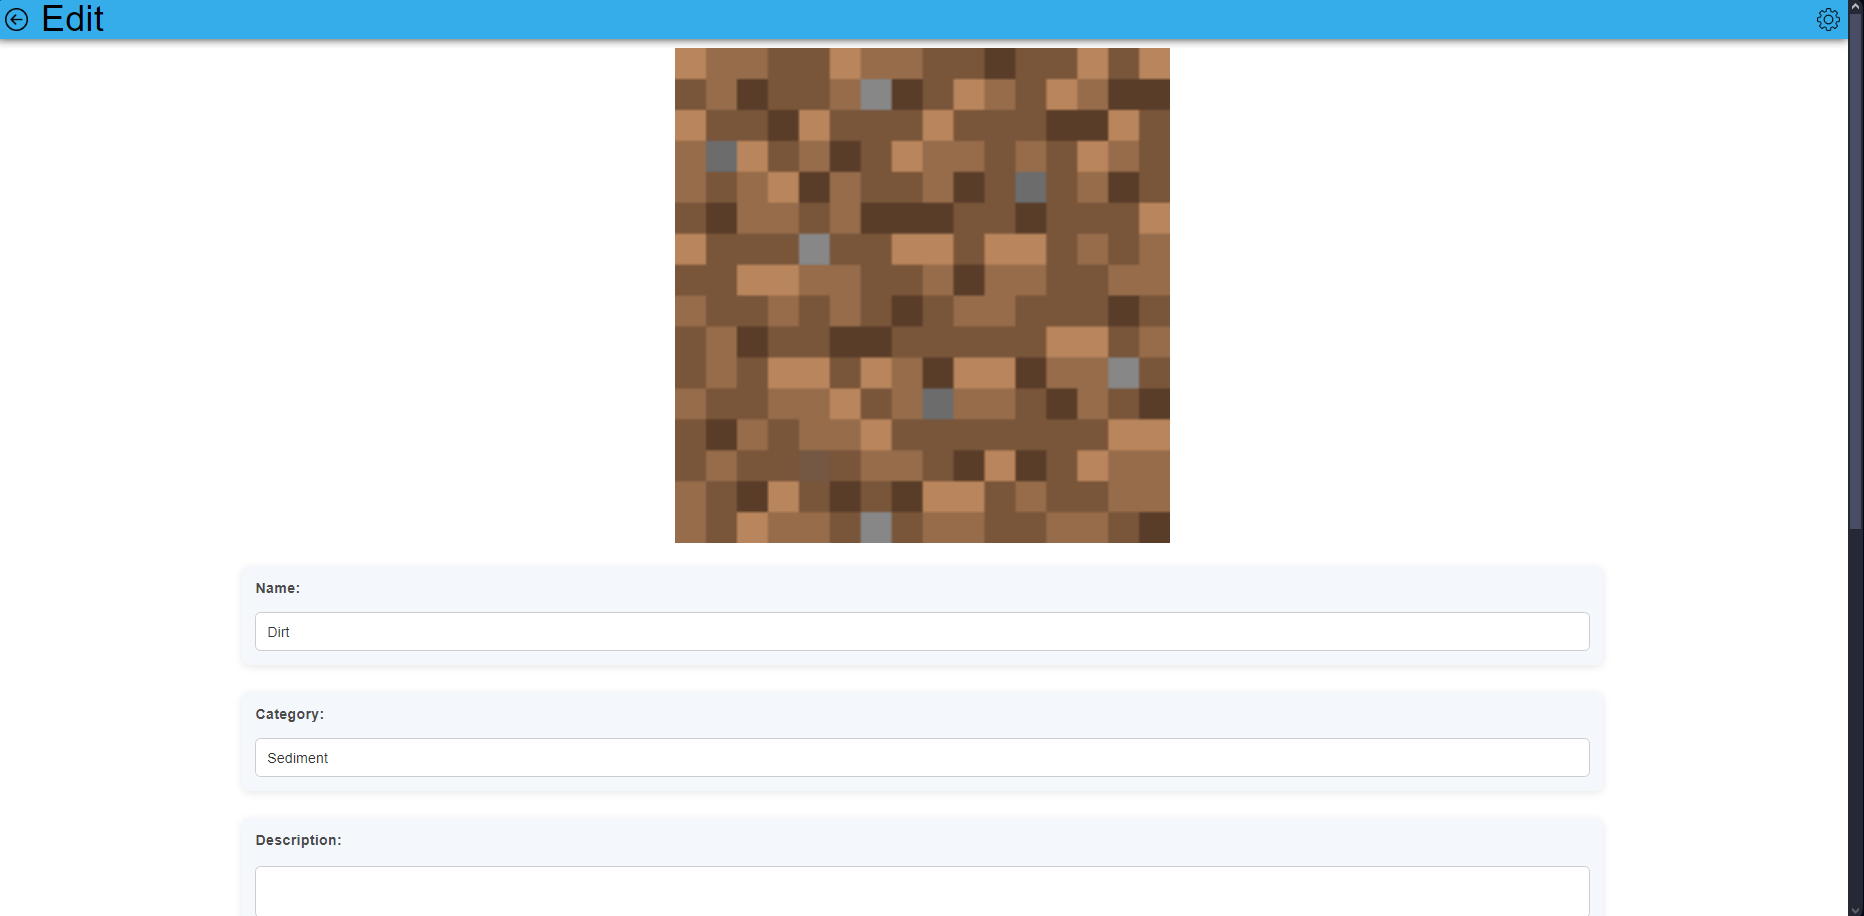
\includegraphics[width=\getImageWidth]{images/app-desktop/app-stock-edit1-desktop.png}
                    \label{fig:app-stock-edit1-desktop}
                \end{subfigure}
                \begin{subfigure}{.49\textwidth}
                    \centering
                    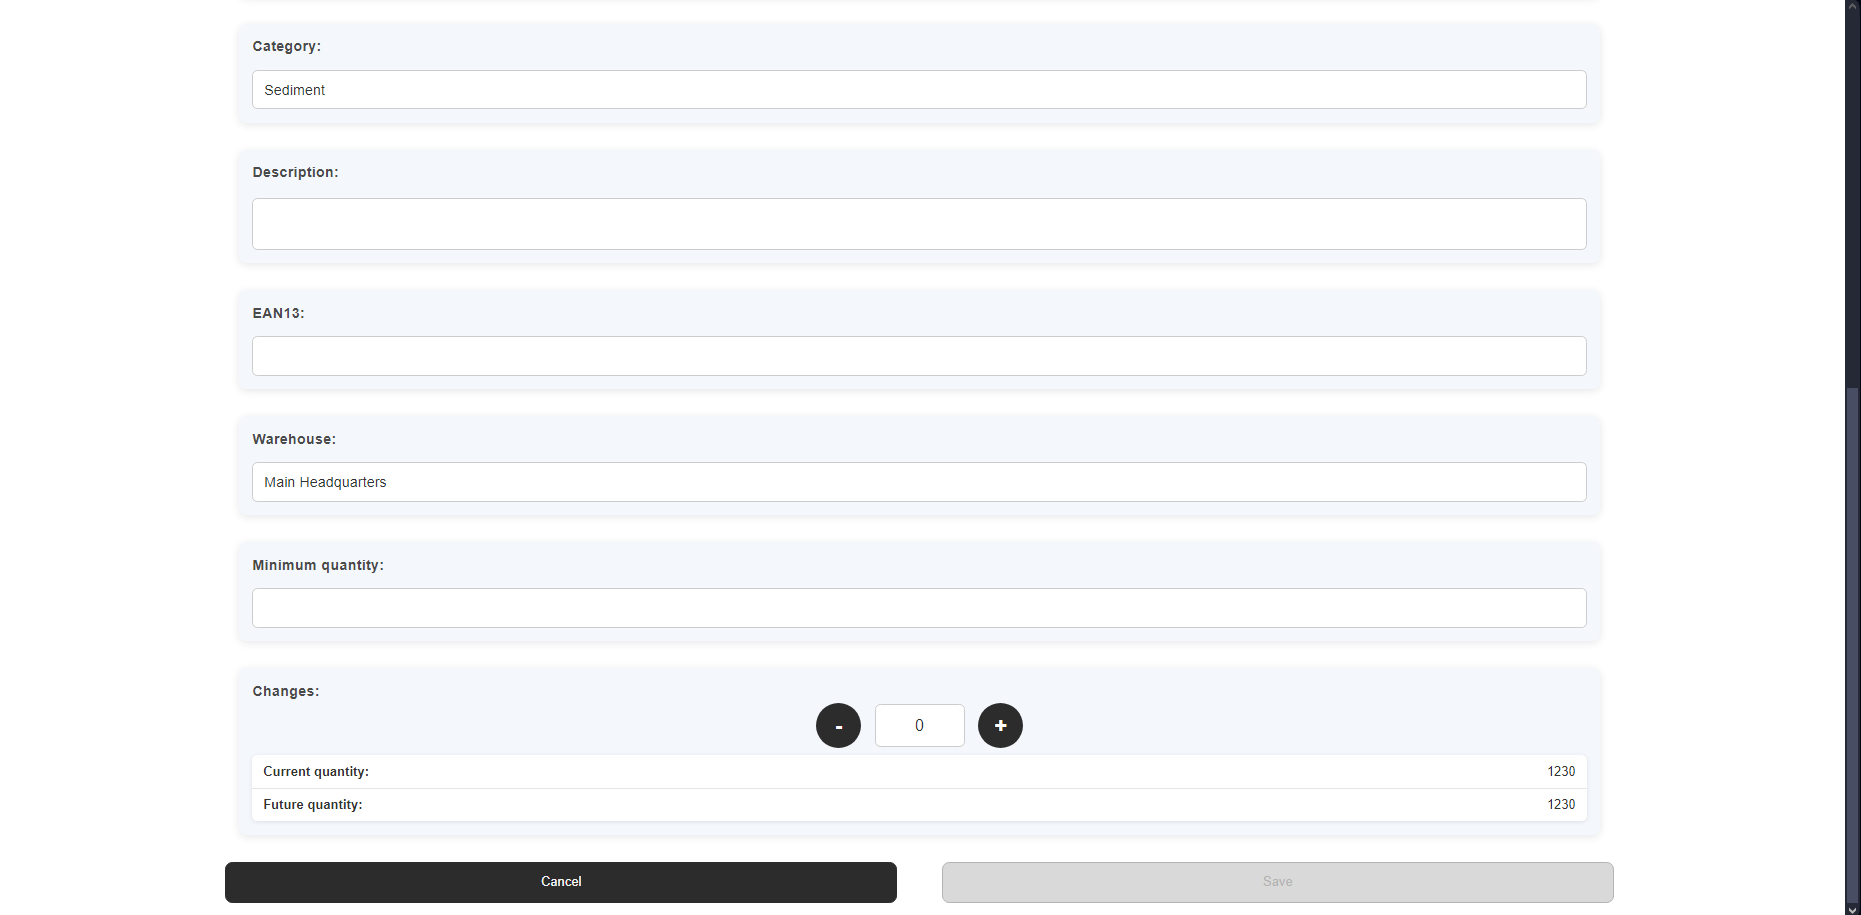
\includegraphics[width=\getImageWidth]{images/app-desktop/app-stock-edit2-desktop.png}
                    \label{fig:app-stock-edit2-desktop}
                \end{subfigure}
                \caption{Widok edycji stanu magazynu}
                \label{fig:app-stock-edit-desktop}
            \end{figure}
            Dodawanie przedmiotu do stanu magazynu działa analogicznie do edycji przedmiotu na stanie magazynu z tą róznicą, że wszystkie pola, poza nazwą aktualnego magazynu, są wstępnie puste.

            \begin{figure}[H]
                \begin{subfigure}{.49\textwidth}
                    \centering
                    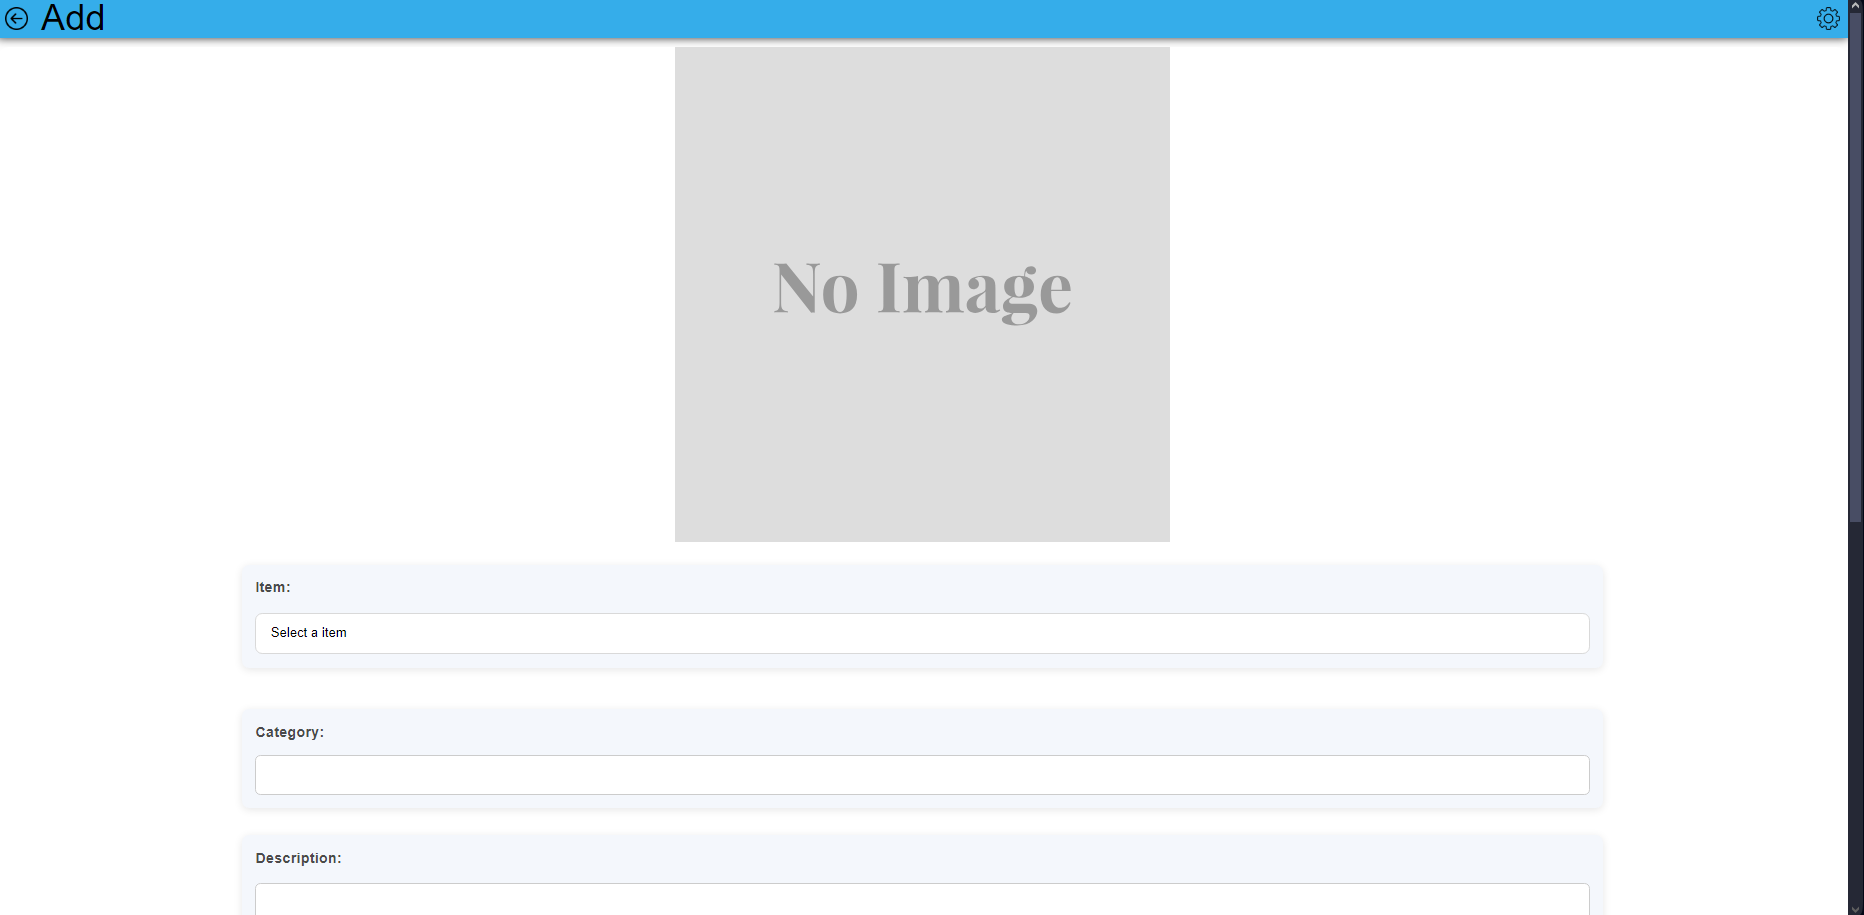
\includegraphics[width=\getImageWidth]{images/app-desktop/app-stock-add1-desktop.png}
                    \label{fig:app-stock-add1-desktop}
                \end{subfigure}
                \begin{subfigure}{.49\textwidth}
                    \centering
                    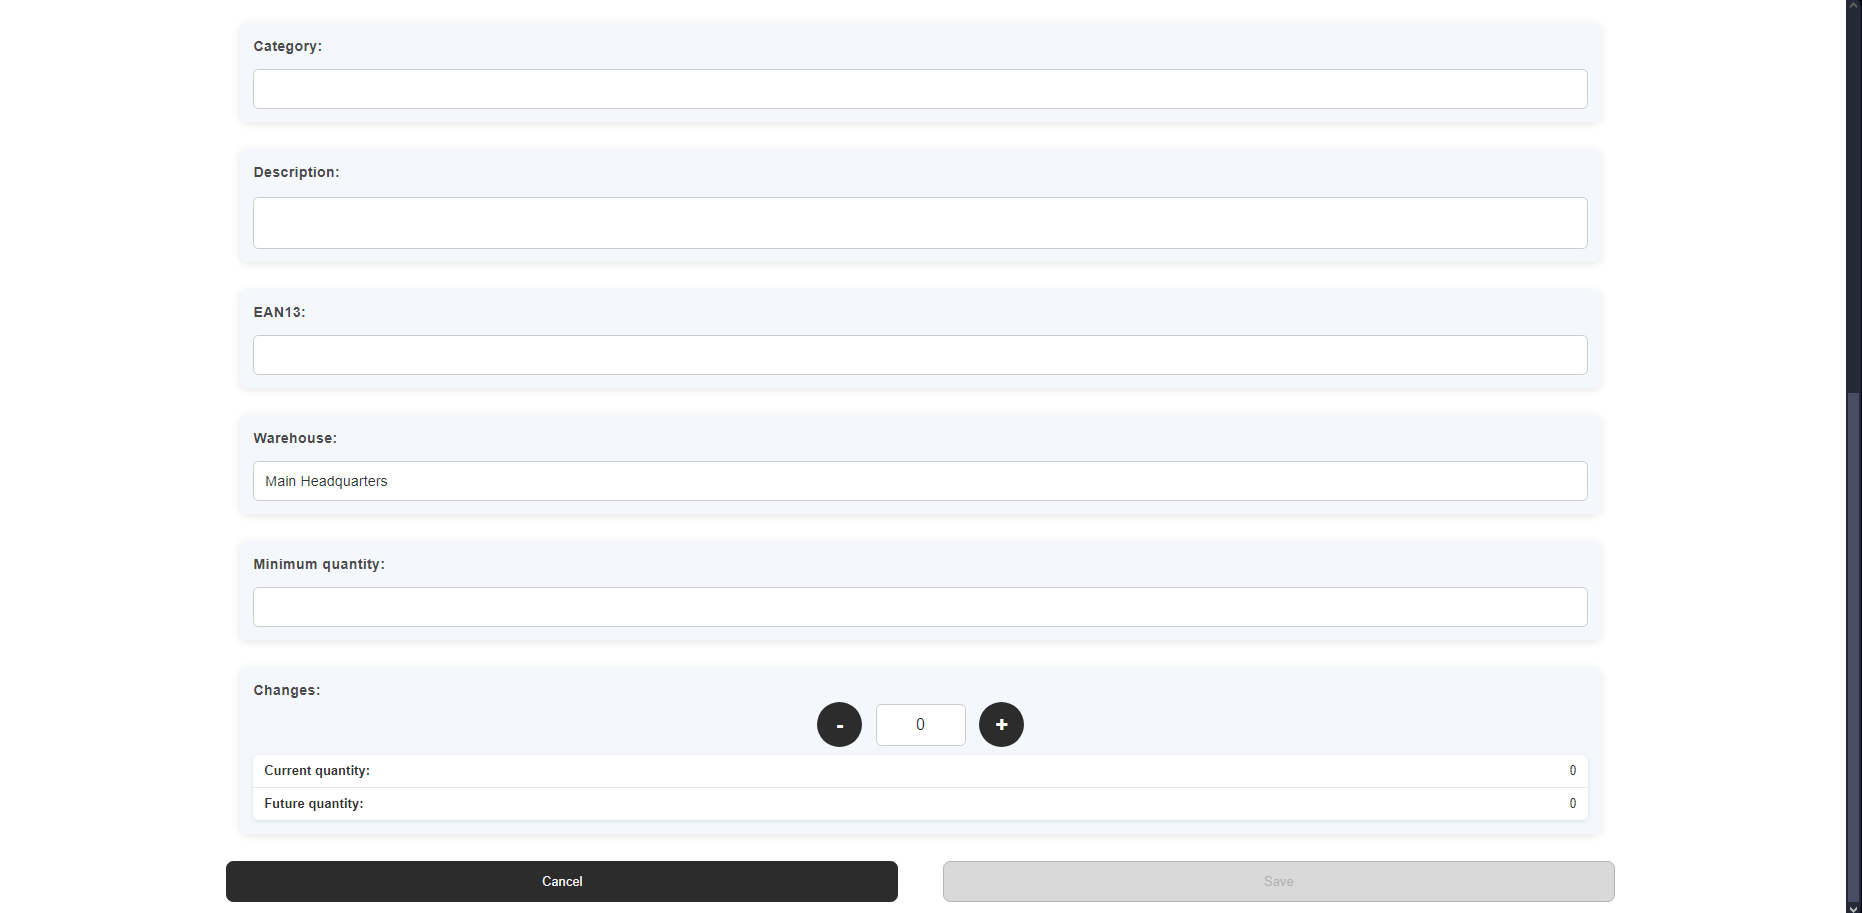
\includegraphics[width=\getImageWidth]{images/app-desktop/app-stock-add2-desktop.png}
                    \label{fig:app-stock-add2-desktop}
                \end{subfigure}
                \caption{Widok dodawania stanu magazynu}
                \label{fig:app-stock-add-desktop}
            \end{figure}

        \FloatBarrier 
        \subsubsection{Skaner}
            Widok skanera przedstawiony jest na Rysunku \ref{fig:app-scanner-mobile} i zawiera tylko obraz z kamery. Po zeskanowaniu odpowiedniego kodu użytkownik zostaje przekierowany do odpowiedniej strony: artykułu - jesli zeskanował kod EAN13; stanu domyślnego magazynu - jeśli zeskanował kod QR z zawartym ID artykułu.

            \begin{figure}[H]
                \centering
                
\includegraphics[height=\getImageHeight]{images/app-mobile/app-scanner-mobile.jpg}
                \caption{Widok skanera kodów kreskowych i kodów QR}
                \label{fig:app-scanner-mobile}
            \end{figure}

\end{document}